\chapter{Proposed Method}
\label{chapter: proposed_method}
\textit{The goal of this chapter is to provide a description of the proposed algorithm and to list tests with expected outcomes which, if implemented provide evidence for the effectiveness of the algorithm. The previous chapter has answered the first 2 research subquestions by showing existing methods and their limitations which have been highlighted. This chapter answers the last research subquestion by providing a draft method to be investigated in the thesis, the method can complete tasks while learning system dynamics during task execution in an environment with movable obstacles. The proposed algorithm relies on many existing methods which have been discussed in \cref{chapter: interaction_with_env_and_model_identification,chapter: task_and_motion_planning} and will be rediscussed briefly in \cref{subsection: required_components}. \Cref{section: hgraph} defines the hypothesis graph, as \cref{section: knowledge_graph} defines the knowledge graph. Benchmark tests are listed in \cref{section: btests}. The Discussion is presented in \cref{section: proposed_method_discussion}.\\}

In this literature study the focus lies on the knowledge graph (KGraph), the hypothesis graph (HGraph) and the robot simulation environment. If the literature study focus would be complemented with a high-level planner and an ontology, the robot framework would be theoretically capable of handling high-level tasks, such as grouping objects based on shape, or cleaning.\\

\textbf{\large general outline\\}
\noindent \Cref{figure: block_framework} displays the general outline control structure for the robot. Upon receiving a task, the \textit{hypothesis graph} is responsible for generating a hypothesis, an action sequence which might lead to successful completion of the given task. Replanning may occur after learning objects are immovable or when control fails to complete a subtask, if all possible hypothesis have been tried, then HGraph concludes that the task cannot be done. \Cref{section: hgraph} is fully dedicated to explaining the hypothesis graph.\\

After execution of an action, the action is evaluated and newly learned knowledge is stored or updated in the \textit{knowledge graph}. Aside from storing knowledge, the knowledge graph provides action suggestions to the hypothesis graph. \cref{section: knowledge_graph} is fully dedicated to explaining the knowledge graph.\\

\begin{figure}[H] \centering
\begin{tikzpicture}[node distance = 2cm, auto]
    % Place nodes
    \node[draw=gray, rounded corners, inner sep=3ex, line width=7pt, fill=gray, fill opacity=0.4, minimum height=12.1cm, minimum width=6.8cm, yshift=3.7cm] (focusbox) {}; 
    \node[yshift=5.5cm, xshift=-0.6cm, align=left] at (focusbox) {\textbf{Literature study focus}};
   
   \node [outer sep=0cm] (environment) at (0,0)  {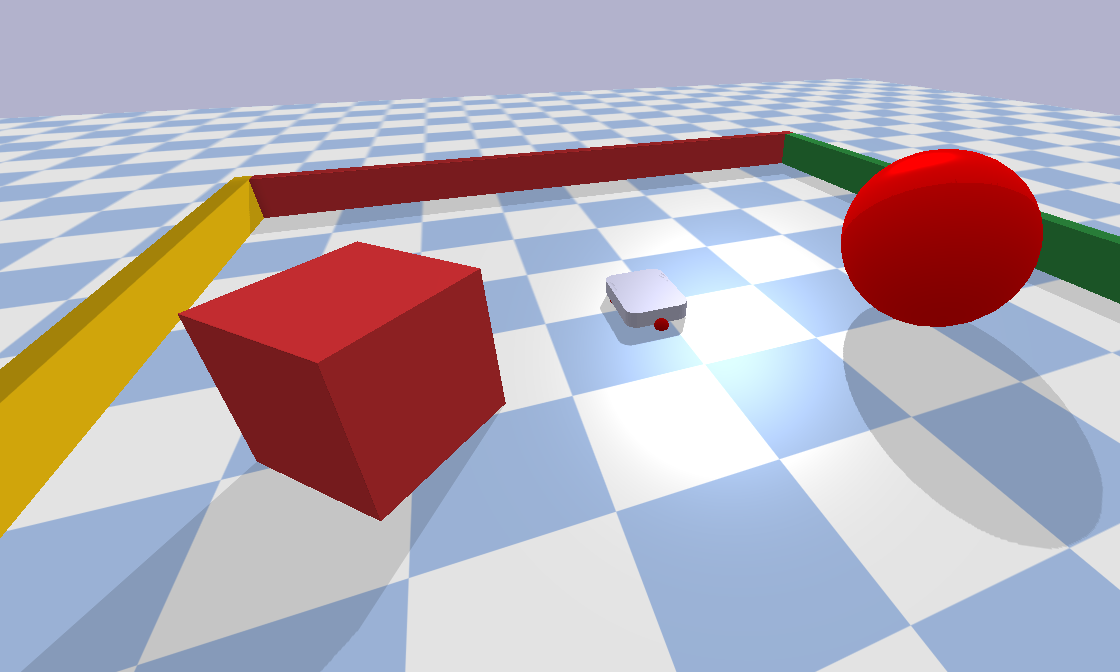
\includegraphics[width=5.0cm]{figures/task_swap_location_balls.png}}; 

   \node [below, xshift=0.2cm, yshift=-.1cm, text width=5cm, align=left, outer sep=0cm] at (environment.north) {\textbf{Robot Environement}};
   
    \draw [myEvenLighterColor,
    rounded corners=0.3cm, 
    line width=0.3cm]  
    (environment.north west) -- 
    (environment.north east) --
    (environment.south east) --
    (environment.south west) -- cycle  ;
    
    \node [block,
    above of=environment,
    minimum height=2cm,
    minimum width=5cm,
    node distance=4.3cm,
    outer sep=0cm] (hgraph) {Hypothesis Algorithm};
   
    \node [block, 
    above of=hgraph, 
    node distance=3.5cm, 
    minimum width=5cm,
    minimum height=2.0cm] (kgraph) {Knowledge Graph};
      
    \node [rectangle, draw, 
    fill=myEvenLighterColor, 
    text width=5em, text centered, rounded corners, 
    right of=kgraph, 
    minimum width=4cm,
    minimum height=2cm,
    node distance=8cm] (ontology) {Ontology};
     
    \node [rectangle, draw, 
    fill=myEvenLighterColor, 
    text width=5em, text centered, rounded corners, 
    right of=hgraph, 
    minimum width=4cm,
    minimum height=2cm,
    node distance=8cm] (planner) {High-level planner};
    
    
    % Draw edges
    \draw[-stealth] ([yshift=0.155cm, xshift=0.4 cm]environment.north) -- node [right] {\shortstack[]{sensor\\measurements}}([xshift=0.4 cm]hgraph.south) ;
    \draw[-stealth] ([xshift=-0.4 cm]hgraph.south) -- node [left] {robot input}([yshift=0.155cm, xshift=-0.4 cm]environment.north) ;
    \draw[-stealth] (planner.west) -- node [pos=0.37, above] {task}(hgraph.east);
    \draw[-stealth] ([xshift=-0.4cm]kgraph.south) -- node [left] {\shortstack[]{action\\suggestions}}([xshift= -0.4cm]hgraph.north) ;
    \draw[stealth-] ([xshift=0.4cm]kgraph.south) -- node [right] {action feedback}([xshift= 0.4cm]hgraph.north) ;
    \draw[-stealth] (kgraph.east) -- node [above, pos=0.63] {\shortstack[]{environment\\knowledge}}(ontology.west);
    \draw[stealth-] ([xshift=0.4cm]ontology.south) -- node [right] {\shortstack[]{query}}([xshift=0.4cm]planner.north);
    \draw[-stealth] ([xshift=-0.4cm]ontology.south) -- node [left] {\shortstack[]{output}}([xshift=-0.4cm]planner.north);
    \draw[stealth-] (planner.south) |- ++ (2,-1) node[near end, above] {\shortstack[]{High-level\\task}};
    \end{tikzpicture}%
    
\caption{Complete control scheme in Flowchart representation.}
\label{figure: block_framework}
\end{figure}

\section{Required Components}
\label{subsection: required_components}
% yes the label says subsection, it actually is a section
This section lists required components used by the proposed method, such as: path-finding algorithms, controllers or system identification methods. The required components are neatly grouped in this section, every component has a specific citation and it is indicated if any modifications must first be applied before it can be used by the proposed method. The required components are minimally explained, and their function and responsibilities are highlighted. \\

\paragraph{Path Non-Existence}
Before motion planning, the HGraph checks path non-existence, more information on path existence can be found in \cref{subsection: path_existence}. As opposed to motion or manipulation planning two simplifications are made: an obstacle (such as the robot or an environment object) is assumed to be holonomic, and only the unmovable objects are actively present in the configuration space, unknown and movable obstacles are ignored. In configuration space, the free space is discretised with a cell size based on the geometry of the robot or object, a graph-based planner then searches to find a path from starting cell toward the target cell, \cref{figure: path_existence_cite} displays a visual explanation of the path non-existence checker. Paper \cite{akella_simple_2008} describes the method applicable to prove path non-existence, if a path is found toward the target position, the cells containing a path will be converted to sample points in configuration space, serving as a warm start for the motion or manipulation planning algorithms. \\

\begin{figure}[H]
    \centering
    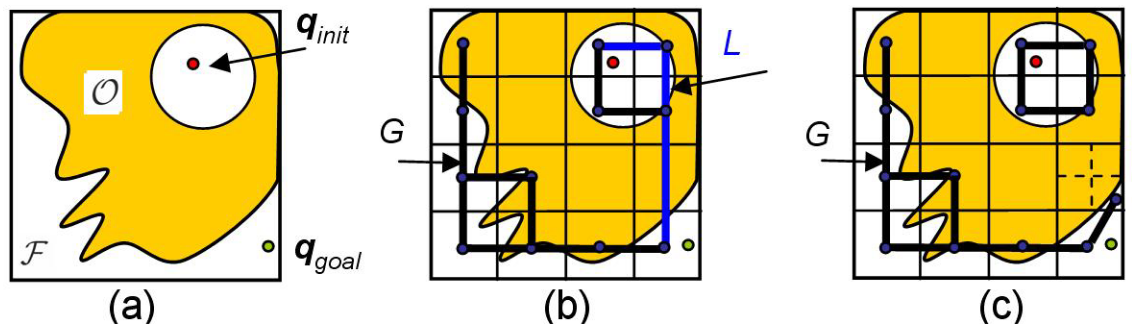
\includegraphics[width=0.8\textwidth]{figures/path_existance_cite.png}
    \caption{Path non-existence between $\text{q}_\text{init}$ and $\text{q}_\text{goal}$. (b): A connectivity graph $G$ is built. The path $L$, which connects the cells including $\text{q}_\text{init}$ and $\text{q}_\text{goal}$, is computed from G. Any mixed cell along $L$ is further subdivided. (c): In the new connectivity graph, the cell containing  $\text{q}_\text{init}$ and the cell containing  $\text{q}_\text{goal}$ are not connected. This concludes that there is no collision-free path between $\text{q}_\text{init}$ and $\text{q}_\text{init}$, From \cite{akella_simple_2008}.}
    \label{figure: path_existence_cite}
\end{figure}

\paragraph{System identification and Control}
In \cref{section: interaction_approaches_and_model_iden_methods} various system identification en control methods have been discussed. Some methods are appropriate candidates for a nonholonomic robot and an environment with movable obstacles. The control and system identification methods are not discussed again here, since they have already been discussed in \cref{section: interaction_approaches_and_model_iden_methods}. The system models generated by system identification methods act as forward models or local planners during motion and manipulation planning as discussed in \cref{section: toward_target_pose,section: toward_sequence_target_poses}.\\
\\

Appropriate candidates for single-body control with system identification methods:
\begin{itemize}
    \item \ac{MPC} control and \ac{PEM} \cite{verhaegen_filtering_2007} system identification
    \item \ac{MPC} control and \ac{IPEM} \cite{seegmiller_vehicle_2013} system identification 
\end{itemize}

A parameterisable system model improves its model accuracy using the \ac{PEM} (offline) or \ac{IPEM} (online) method, the \ac{MPC} controller however keeps constant parameters such as control horizon and the weight matrices. To have some variation in these constant parameters, the robot has access to multiple \ac{MPC} controllers with various control parameters. \\

Appropriate candidates for multi-body system identification and control are:
\begin{itemize}
    \item Reactive \ac{MPC} which requires a single- and multi-body model \cite{toussaint_sequence--constraints_2022}
    \item \ac{MPC} controller and model fitting a 3D-Gaussian \cite{mericli_push-manipulation_2015}
    \item \ac{MPPI} controller and uncertainty calibrated forward model \cite{arruda_uncertainty_2017}
    \item \ac{RMPPI} controller and a \ac{LSTM} \cite{cong_self-adapting_2020}
\end{itemize}

\paragraph{Motion and Manipulation planning}
Finding paths between starting and target configurations is performed by a sampling-based method, a double tree $\text{RRT}^*$ search algorithm \cite{chen_fast_2018}, which searches the configuration space for an optimal path toward the target position. A connectivity graph, (initially only the start and target configuration) keeps track of the configurations reachability from the start and target configuration. Randomly sampled samples are compared to some nearest nodes inside the connectivity graph, before adding the newly sampled node, a check is performed by a local planner to validate if constraints are satisfied, if the random sampled configuration is not valid, it is discarded. The connectivity graph grows from the target configuration and the start configuration, when the connectivity graph from start to target is connected a path is found, pseudocode can be found in \cref{pseudocode: rrt_star}.\\

Manipulation planning is similar to motion planning. With motion planning, planning for the robot is performed, with manipulation planning, planning for the objet to push is performed (and the robot is neglected, but kept track of). So manipulation planning only happens as motion planning for the pushable object.\\

The robot configuration is manipulation planning is kept to validate the reachability to newly sampled samples. To elaborate, adding a new sample is accomplished by, sampling a new configuration for the object to manipulate, the sample is placed in configuration space, with a manually tuned metric function samples nearby the new sample are gathered. A local planner validates if these gathered samples are reachable from the new sample. One configuration is reachable from another configuration if for some input and some system model, one configuration becomes the other configuration in a small amount of time (e.g. $<5$ time steps) an example of such a system model is displayed in \cref{equation: differential_equation_differential_robot}. The difference in predictor between motion (single-body predictor) and manipulation planning (multi-body predictor) thus resides in the local planner and where local motion planner requires 2 configurations, manipulation planning  additionally requires at least one robot configuration. To check if 2 configurations are reachable for manipulation planning 2 object configurations and 1 robot configuration is required, if reachable and connected, an extra robot configuration is generated as a result of the local planner, which is needed for checking reachability of future samples, an visual example is displayed in \cref{figure: local_planner_manipulation}. A manipulation path from start to target will have both the objects and the robot's configurations, where the robot configurations only serve the local planner to validate if two object configurations can be connected. Additionally the robot's path should not collide with obstacles, which needs to be checked during planning. \\

\begin{figure}[H]
    \centering
    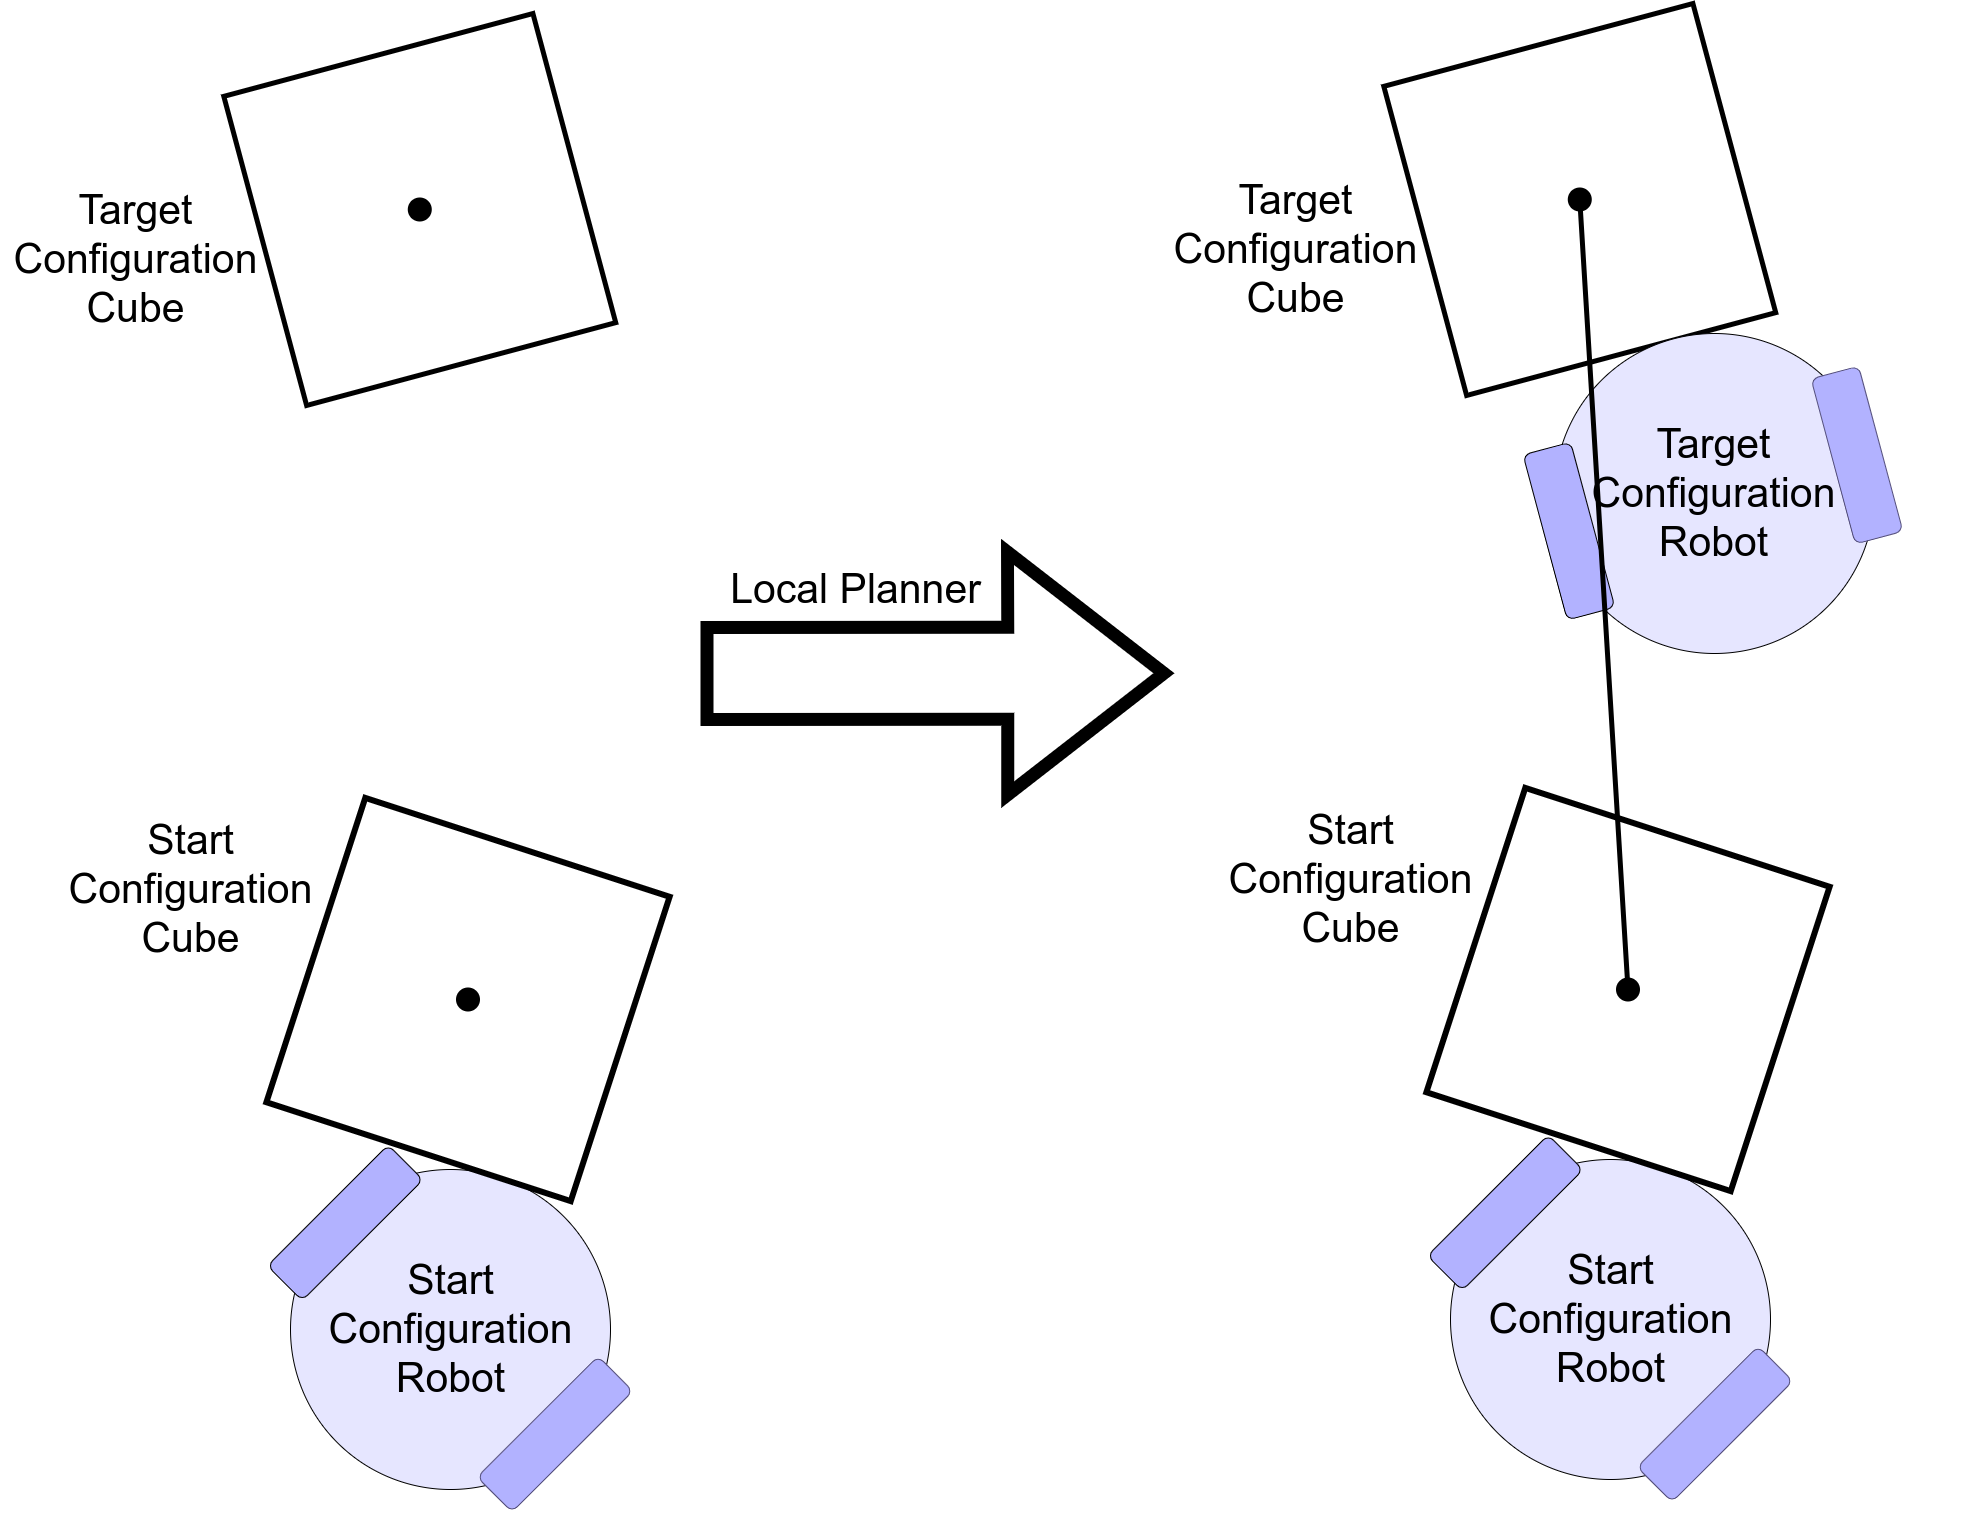
\includegraphics[width=0.7\textwidth]{figures/manipulation_local_planner.png}
    \caption{Local planner connecting 2  cube configurations and generating an new robot configuration}
    \label{figure: local_planner_manipulation}
\end{figure}

The $\text{RRT}^*$ algorithm takes a cost for path length into account, resulting in finding the shortest path with infinite samples if a path exists, an additional cost is added if the path overlaps with a movable or unknown obstacle, motivating the algorithm to find a path around unknown or movable obstacles, but to plan through the obstacles planning around is impossible or costs more. If a path overlaps with an obstacle, a subtask is created to first remove the obstacle, and then continue to track the path. \Cref{figure: double_rrt_alg} gives a visual view of the proposed $\text{RRT}^*$ algorithm.\\

\begin{figure}[H]
    \centering
    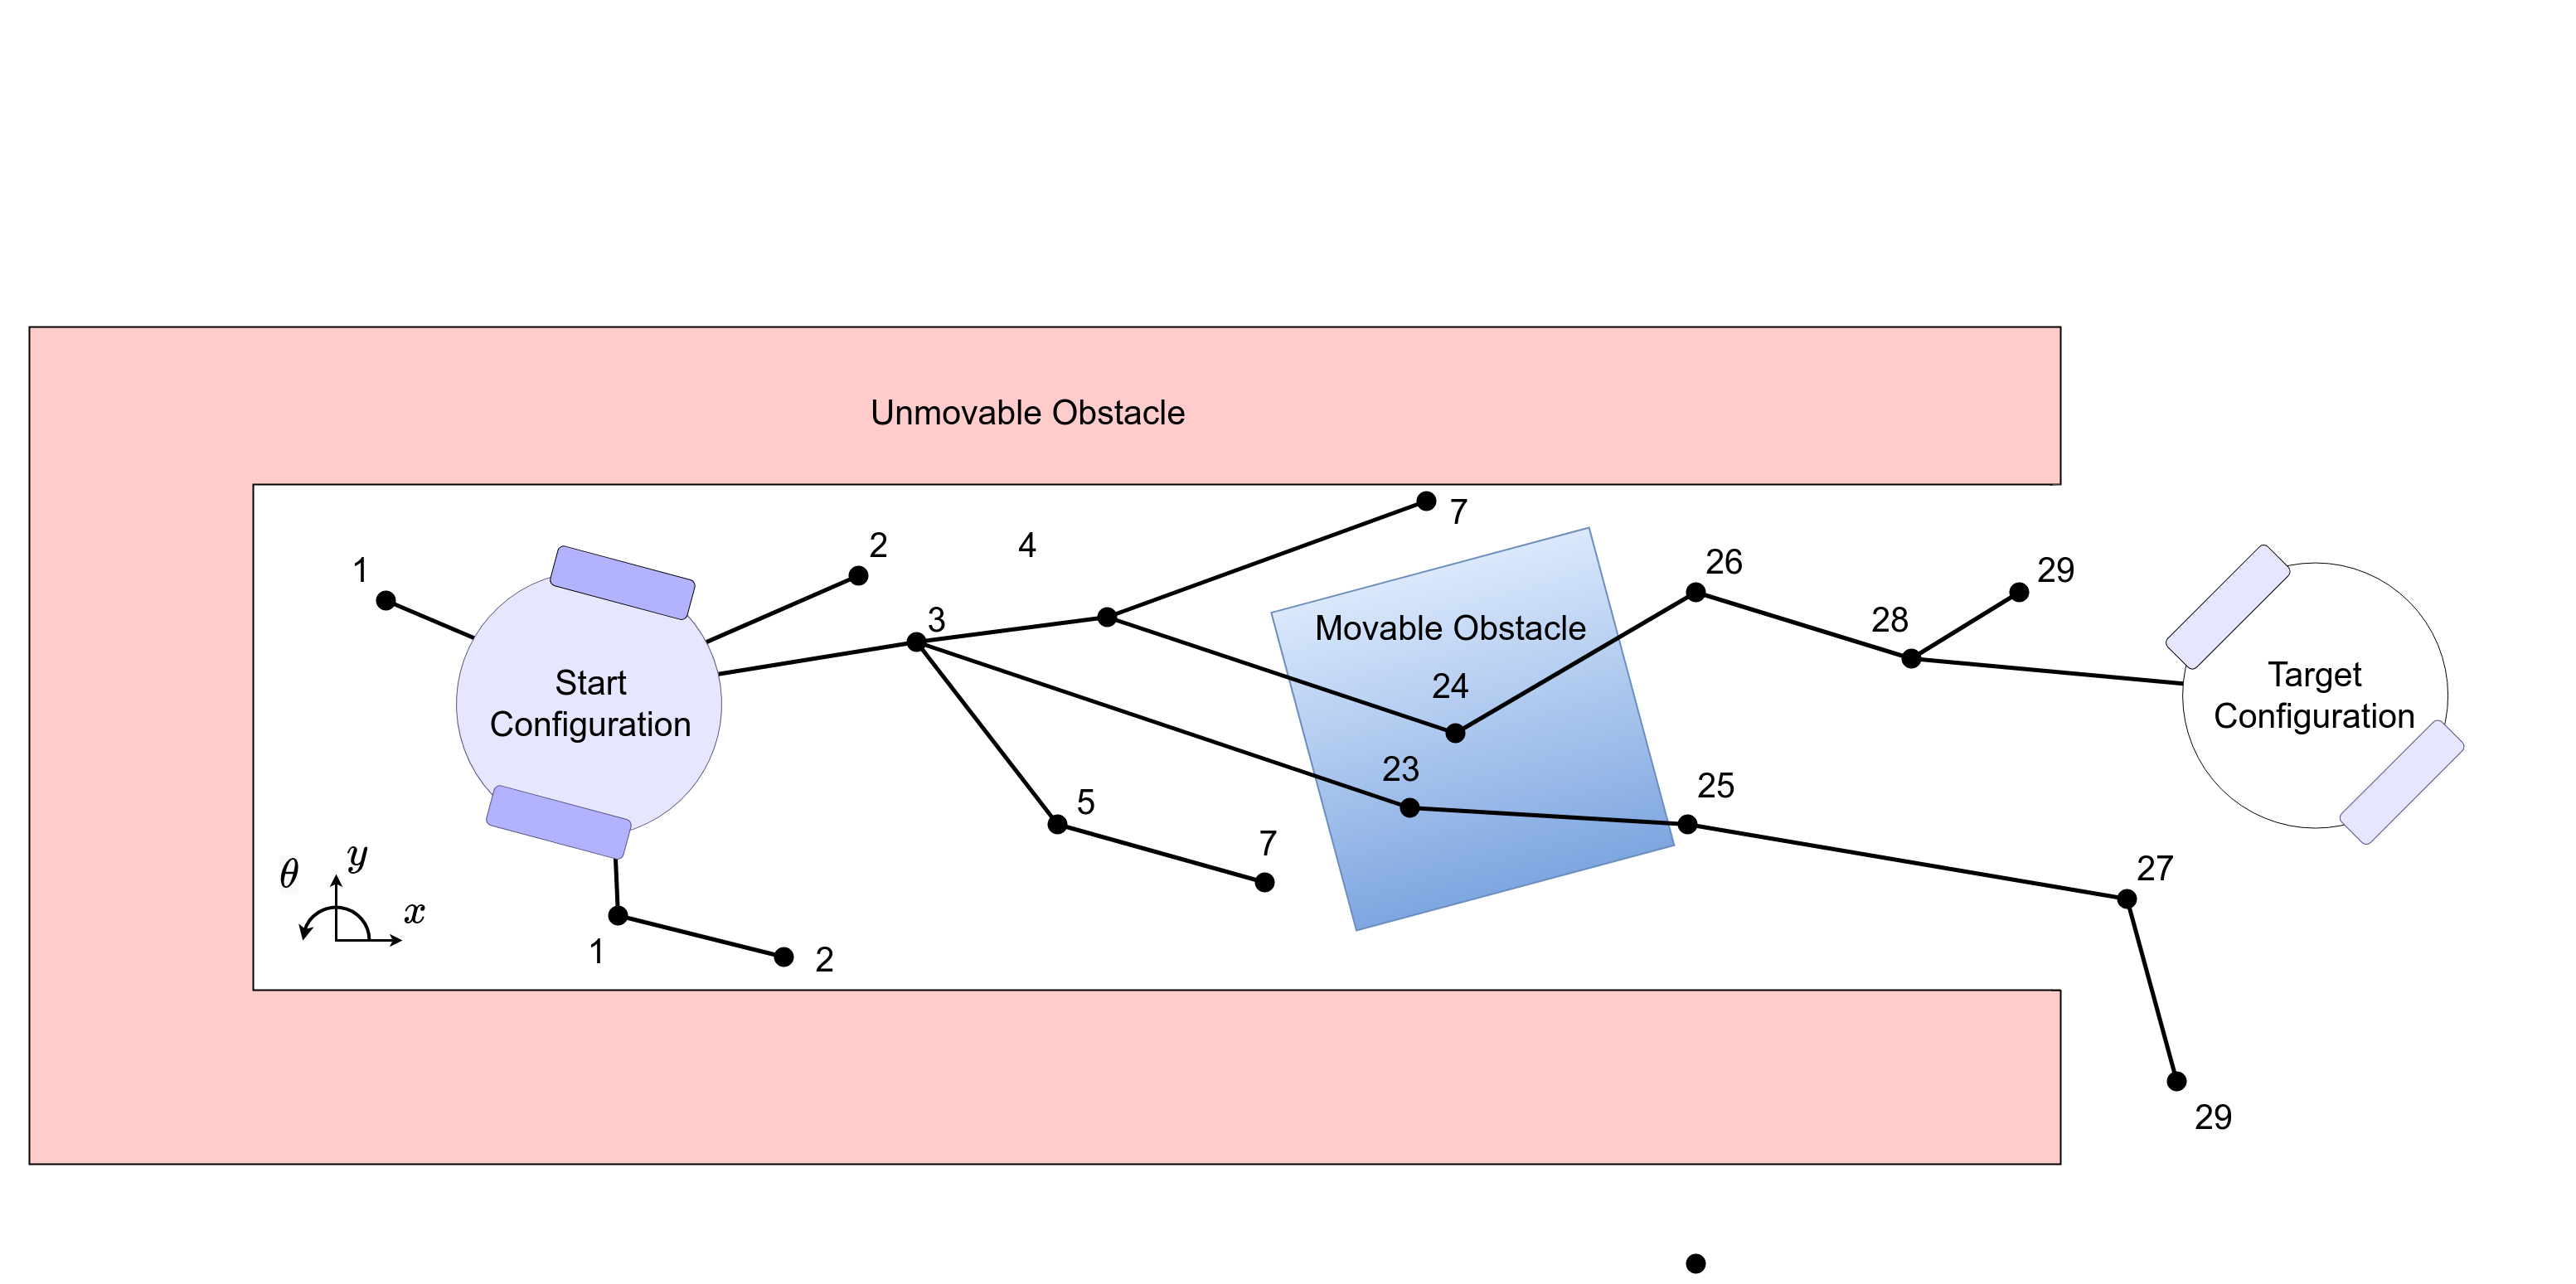
\includegraphics[width=0.9\textwidth]{figures/rrt_with_costs.png}
    \caption{Schematic view of the proposed double $\text{RRT}^*$ tree taking movable and unknown obstacles into account with cost to reach a sampled configuration displayed.}
    \label{figure: double_rrt_alg}
\end{figure}

Note that it remains hard to make predictions on the height of the cost because the object has unknown dynamics, which is why there is a fixed cost for unknown and movable obstacles, unmovable obstacles are captured by the obstacle space. \\

Algorithms \cref{pseudocode: rrt_star} displays the pseudocode for the double $\text{RRT}^*$ algorithm which takes unknown and movable obstacles into account. The following definitions are used by the $\text{RRT}^*$ algorithm. \\

$V$: A set of vertices \\
\indent $E$: A set of edges\\

The following functions are called by the \cref{pseudocode: rrt_star}.\\ 

\noindent $x_{init}$: Creates a start and target configuration. \\ $NotReachStop$: Returns true if the stopping criteria is not reached. \\ $Sample_{free}$: Creates a random sample in free space, free space includes the movable and unknown obstacles. \\ $Nearest(x, V)$: Finds the nearest vertices using euclidean distance \\ $NearestSet(x, V)$: Find a set of nearest vertices using euclidean distance \\ $Project(x, x')$: Project $x'$ toward $x$ such that it lies close enough to a vertices to be compared using a local planner \\ $CollisionCheck(x)$: returns true if $x$ is in free-space, movable obstacle or unknown obstacle \\  $CostFromInit(x, x')$: Find the total cost from $x$ to the initial vertices via $x'$, cost is determined as a sum of path length and if the path overlaps with movable of unknown objects. \\ $ConstraintsCheck(x, x')$: return true if a local planner is able to connect $x$ and $x'$ using a forward model. \\

\begin{algorithm}[H]
\caption{Proposed Double tree $\text{RRT}^*$ algorithm taking movable obstacles and constraints into account, edited $\text{RRT}^*$ pseudocode from \cite{chen_fast_2018}}
\label{pseudocode: rrt_star}
\begin{algorithmic}[1]
\State $V \leftarrow x_{init}$
\While{$NotReachStop$} 
    \State $Cost_{min} \leftarrow +\infty$
    \State $x_{rand} \leftarrow Sample_{free}$
    \State $x_{nearest} \leftarrow Nearest(x_{rand}, V)$
    \State $x_{temp} \leftarrow Project(x_{nearest}, x_{rand})$
    \If{$CollisionCheck(x_{temp}) == True$}
        \State $x_{new} = x_{temp}$
        \Else
        \State $Continue$
    \EndIf
    \State $X_{near} \leftarrow NearestSet(x_{new}, V) $
    \For{$x_{near} \in X_{near}$}
        \If{$CostFromInit(x_{new}, x_{near}) < Cost_{min}$}
            \If{$ConstraintsCheck(x_{new}, x_{near}) == True $}
            \State $Cost_{min} \leftarrow CostFromInit(x_{new}, x_{near})$
            \State $x_{minCost} \leftarrow x_{near}$
            \EndIf
        \EndIf
    \EndFor
    \If{$Cost_{min} != \infty$}
        \State $V.add(x_{new})$
        \State $E.add(x_{minCost}, x_{new})$
    \EndIf
\EndWhile
\end{algorithmic}
\end{algorithm}

\paragraph{Notation standard}
For the upcoming \cref{section: hgraph,section: knowledge_graph}, especially for the definitions of the hypothesis and knowledge graph a notation standard is used. A list of hypothesis and knowledge graph related symbols is shown in \cref{table: symbol_list_hgraph}.\\

Subscripts are used to indicate what the variable belongs to. For example, the state variable of the robot is written down as $s_{robot}$. Certain variables indicate the same object, but with different values, this is indicated by different superscripts. For example $s_{robot}^1$ and $s_{robot}^2$ are different states but both indicate the robot's state, formally $||s_{robot}^1-s_{robot}^2|| \neq 0$. $k$ indicates the time step, for example, the state of the robot at time step $k$: $s_{robot}(k)$. For convenience, the time step index is sometimes dropped. \\ 

\renewcommand{\arraystretch}{1.2}
\begin{table}[H]
    \centering
    \begin{tabular}{p{2cm} l }
        $k$ & \textrm{time step index}\\
        $s_{id}(k)$: & \textrm{State}\\
        $c_{id}(k)$: & \textrm{Configuration}\\
        $\mathcal{C}_{id}(k)$: & \textrm{configuration set}\\
        $ob_{id}(k)$: & \textrm{Object}\\
        $\mathcal{O}_{id}(k):$ & \textrm{Object set}\\
        $V^{ob}_{id}$: & \textrm{node storing set of objects}\\
        $V^{conf}_{id}$: & \textrm{node storing set of configurations}\\
        $V^{\Delta conf}_{id}$: & \textrm{node storing set of configurations and boolean lists}\\
       $d$: & \textrm{dynamical model}\\
        $\alpha$: & Success factor\\
        $\tau_{(i,j)}$: & \textrm{Transition}\\
        $G^{knowledge}$: & \textrm{knowledge graph}\\
        $G^{hypothesis}$: & \textrm{hypothesis graph}\\
        $h$: & \textrm{plan, hypothesis}\\
        $path$: & \textrm{list of configurations indicating a path, or False}
   \end{tabular}
    \caption{List of symbols used in the hypothesis- and knowledge graph, where $id$ is a unique identifier of the object}
    \label{table: symbol_list_hgraph}
\end{table}

\section{Hypothesis Graph}%
\label{sec:hgraph}
The \ac{halgorithm} is responsible for generating action sequences, called hypothesis. An hypothesis consists of a list of successive edges in the \ac{hgraph} from start to target node in the \ac{hgraph}. When all subtasks in a task are completed, the \acf{halgorithm} halts and concludes the task successfully completed. A search in the joint configuration space is avoided because an edge only operates in a single mode of dynamics, such as driving or pushing. When an object cannot directly be steered toward its target location new nodes are generated which need to be completed before the original object can be steered toward its target location. An example of when an object cannot directly be steered toward its target state is because the path is blocked by another object. A hypothesis, consisting of a list of edges that represent actions in the robot environment might succeed or fail. \Cref{tikz:flowchart_hgraph} displays a flowchart explaining how new nodes and edges are generated in the \ac{hgraph}. Successfully completed edges eventually result in completed subtasks, failed edges trigger replanning that will restart the search to a hypothesis.\bs

The \ac{halgorithm} with the \ac{hgraph} have a familiar structure compared to some recent literature~\cite{ellis_navigation_2022,wang_affordancebased_2020}. An important distinction is that the proposed method in this thesis aims to combine the 3 topics: learning object dynamics, solving \ac{NAMO} problems and nonprehensile pushing. Recent literature is able to only combine one or two topics of the three.\bs

In the upcoming section the \ac{hgraph} is defined and discussed in \cref{subsec:hgraph_definition}. The \ac{halgorithm} is then discussed and in \cref{subsec:halgorithm}, where an explanation is provided on how the \ac{halgorithm} searches for a solution in the joint configuration space. The section is concluded with an extensive example.\bs

\subsection{Definition}%
\label{subsec:hgraph_definition}%
Before defining the \ac{hgraph}, some definitions are defined on which the \ac{hgraph} depends. First, recall the \textbf{state} defined in the \cref{sec:problem_description}.\bs

An object holds the information about an object.\\Formally, a \textbf{object},  $obst_{id}(k) = \left\langle s(k), shape \right\rangle $\bs

where $shape$ is linked to a 3D representation of the object which is used to construct the configuration space.\bs

An object node represents an object in a state.\\Formally, a \textbf{objectNode}, $V^{obst}_{id} =\left\langle \textrm{status}, obst(k)\right\rangle $\\where status indicates if the node has been visited in the \ac{hgraph}. $\textrm{status} = (Initialised, Completed, Failed)$\bs

An edge describes the details of how a node transitions to another node in the \ac{hgraph}. In the robot environment, an edge represents a change of state for an object. System identification and performing an action such as pushing or driving both change the state of objects in the robot environment, but because are very different, the edges are split into 2 categories. IdentificationEdges that collect system \ac{IO} data and convert that into a system model. And actionEdges that plan and track a motion from a start to a target state. Formally:\bs

A \textbf{identificationEdge},
\todo[inline]{define identificationEdge, currently hard coded models are used in the implementation}

A \textbf{actionEdge}, $\tau_{(from, to)} = \left\langle \textrm{status}, id_{from}, id_{to}, \textrm{verb}, \textrm{controller},\textrm{dynamic model}, \textrm{path}\right\rangle$\bs

with $id_{from}$ and $id_{to}$ indicating the node id of the node in the \ac{hgraph} where the edge start from and point to respectively, $verb$ an English verb describing the action the edge represents, the controller contains the controller used for driving the robot, the dynamic model is the dynamic model used by the controller, path a list of configurations indicating the path connecting a start- to target node.\bs
\todo[inline]{Martijn: what does this mean: "the controller contains the controller..."?}

A $verb = \{\textrm{driving, pushing}\}$.\bs

Now the nodes and edges have been defined, the \ac{hgraph} can be defined.\bs

Formally, a \textbf{hypothesis graph}, $G^{hypothesis} = \left\langle V, E \right\rangle $ 
\\comprising $V = \{V^{ob}_{i}\}$, \quad $E \in \{\tau_{(i,j)}| V_i, V_j \in \{V^{ob} \}, i \neq j\}$.\bs

Most \ac{hgraph} components have now been defined. The status of an identification edge or action edge still remains undefined and requires some further explanation.\bs

\paragraph{Status, Types and Lifetime of edges}
Because system identification and tracking a path are so very different, the edges are split into two categories, identification edges and action edges. An identification edge, which is responsible for sending an input sequence to the system and recording the system output. That input/output sequence and assumptions on the system are the basis for system identification, techniques on various system identification methods are discussed in \cref{sec:sys_iden}. The goal is to create a dynamical model which is augmented with a corresponding controller is closed-loop stable.\bs

An identificationEdge, the status can be visualised in \cref{tikz:status_identification_edge}.\bs

\begin{figure}[H]
\centering
\begin{tikzpicture}[node distance = 2cm, auto, initial]
    \node [state, fill=my_dark_blue] (init_test_num) {IT\#t};
    \node [state, fill=my_light_blue, below of=init_test_num] (completed_test_num) {CT\#t};
    \node [state, accepting, fill=my_green, below of=completed_test_num] (completed) {CO};
    \node [state, accepting, fill=my_red, right of=completed_test_num, node distance=6cm] (failed) {FAIL};

 % arrows
    \draw [-stealth] ([xshift=-2cm]init_test_num.west) to node[near start,above]{\shortstack[]{select compatible\\sys. iden. method}} (init_test_num.west);
    \draw[-stealth] (init_test_num) edge[bend right] node[left]{Collect \ac{IO} data} (completed_test_num)
(completed_test_num) edge node[left]{create system model} (completed);
    \draw [-stealth] (completed_test_num) edge[bend right] node[right]{goto next start state} (init_test_num);
    \draw [-stealth] (completed_test_num) to node[]{Unable to reach next start state}  (failed.west);
    \draw [-stealth] (init_test_num) [out=0, in=90] to node[above]{Unable to reach next pos}  (failed.north);

\end{tikzpicture}
\caption{\acs{FSM} displaying the status of an identification edge}%
\label{tikz:status_identification_edge}
\end{figure}

\todo[inline]{some explainer on this status of iden edge}

The second type of edge is an actionEdge, containing a drive or push action. An actionEdge ready for execution contains all the necessary information to send input to the robot resulting in an object being steered toward it's target state. Before an edge is ready for execution it should be initialised properly, more specifically: initialised, path estimated should be performed, a system model must be initiated and path planning must be performed. Then finally the edge is ready to be executed and send input toward the robot, an \ac{FSM} of the actionEdge's status can be visualised in \cref{tikz:status_action_edge}.\bs

\begin{figure}[H]
\centering
\begin{tikzpicture}[node distance = 2cm, auto, initial]
    % \node [state, fill=lavenderIndigo] (init) {IN};
    \node [state, fill=my_purple] (init) {IN};
    \node [state, fill=my_dark_blue, below of=init] (path_exist) {PE};
    \node [state, fill=my_light_blue, below of=path_exist] (system_model) {SM};
    \node [state, fill=my_green, below of=system_model] (path_planned) {PP};
    \node [state, fill=my_yellow, below of=path_planned] (executing) {EX};
    \node [state, accepting, fill=my_orange, below of=executing] (completed) {CO};
    \node [state, accepting, fill=my_red] (failed) at ([xshift=4cm]$(system_model)!0.5!(path_planned)$) {FAIL};
    
 % arrows
    \draw [-stealth] ([xshift=-2cm]init.west) to node[near start,above]{select controller} (init.west);
    \draw[-stealth] (init) edge node[left]{graph-based path estimation} (path_exist)
      (path_exist) edge[bend right] node[left]{load in system model} (system_model)
(system_model) edge[bend right] node[left]{motion planning} (path_planned)
(path_planned) edge[bend right] node[left]{goto execution loop} (executing)
(executing) edge[bend right] node[left]{completed} (completed);

    \draw [-stealth] (init.east) [out=0, in=90] to node[xshift=0.1cm, right]{path non-existence proven}  ([yshift=-0.03cm,xshift=0.2cm]failed.north);
    \draw [-stealth] (path_exist.east) [out=0, in=90] to node[xshift=-0.6cm,yshift=0.55cm, above]{\shortstack[l]{system\\identification\\error}}  ([yshift=-0.03cm,xshift=-0.2cm]failed.north);
    \draw [-stealth] (system_model.east) [out=0, in=180] to node[xshift=0.1cm, yshift=0.3cm, above]{\shortstack[l]{motion\\planning\\error}} (failed.west);
    node[right]{motion planning error}  
    ([yshift=-0.3cm]failed.west);
    \draw [-stealth] (executing.east) [out=0, in=-90] to node[xshift=0.1cm,right]{fault detected}(failed.south);

\end{tikzpicture}
\caption{\acs{FSM} displaying the state of an action edge}%
\label{tikz:status_action_edge}
\end{figure}

% \par\smallskip\noindent
\centerline{\begin{minipage}{0.8\textwidth}
\begin{enumerate}
  \item[INITIALISED (IN)] The edge is created with a source and target node which are present in the \ac{hgraph}. A choice of controller is made.
    \item[PATH EXISTS (PE)] A graph-based search is performed to validate if the target state is reachable assuming that the system is holonomic.
    \item[SYSTEM MODEL (SM)] A dynamics system model is provided to the controller residing in the edge.
    \item[PATH PLANNED (PP)] Resulting from a sample-based planner, a path from start to target state is provided. 
    \item[EXECUTING (EX)] The edge is currently receiving observations from the robot environment and sends back robot input. 
    \item[COMPLETED (COMPL)] The edge has driven the system toward its target state and its performance has been calculated.
    \item[FAILED (FAIL)] An error occurred, yielding the edge unusable. 
\end{enumerate}
\end{minipage}}
\par\smallskip

\Cref{tikz:status_action_edge} shows that many steps must successfully be completed before the robot can start executing. The performance of an edge during execution, measured in various metrics (\cref{sec:proposed_method_metrics} is dedicated to metrics) is dependent on many aspects. Such as the choice of controller, the path estimation, the system model yielded by the identification edge and the path yielded by motion planning. Now that he \ac{hgraph} is defined, let's see how it is generated in the upcoming section.\bs

\subsection{\acl{halgorithm}}%
\label{subsec:halgorithm}
This section will provide a mathematical description of the proposed \ac{halgorithm}, the search and execution loop are discussed. The section will finalise with 4 examples. First, let's look into the math of the \ac{halgorithm}.\bs

\todo[inline]{a mathematically solid describtion of your backward search algorithm}

During a backward search, edges are added pointing toward the target node (or to nodes that point toward the target node). Trying to connect the robot node through a list of succesive directed edges to a target node. If such a path has been found in the \ac{hgraph}, a hypothesis has been found and the robot can start executing edges.

A flowchart of the \ac{halgorithm} is presented in \cref{tikz:flowchart_hgraph}. Compared to the mathematical description of the \ac{halgorithm} the flowchart provides more detail, including an eleborate description for every block in the flowchart (see \cref{table:explainer_hgraph_figures_nodes}). The flowchart includes path estimation, planning and the behavior when failure occures. A connection point to the \ac{kgraph} and robot environment are included. The blocks in the flowchart indicate which action they take and where, such as the configuration space, the \ac{kgraph} or the \ac{hgraph}. With the flowchart is straigtforward to see how the \ac{halgorithm} connects to the status of edges, with the mathematical description of the \ac{halgorithm} that is harder so see. Compared to the flowchart the mathematical description is a abstacted version, leaving many details out that are related to the robot in this thesis. An abstracted mathematical description is simpler and encompasses a broader field of robots. So could the mathematical description also be applied to another robot such as a movable robot with robot arm and gripper. The flowchart encompasses to many details to be applied after such an change in robot hardware. 

% \newgeometry{left=1.1cm,bottom=0.1cm,top=1.9cm,headsep=0.1in,heightrounded}

\newpage
\vspace*{-1.2cm}
\hspace{-1.2cm}
\begin{minipage}{10cm}
\begin{figure}[H] 
\centering
\begin{tikzpicture}]
  [node distance = 3cm] 

    % Nodes
    \node [block, fill=yellow!50, line width=2pt, dashed] (first) {Create Start and Target Nodes};
    
    % legend
    \node[text width=2.8cm, yshift=0.6cm, right of=first, node distance=7cm, text centered, rounded corners, minimum height=1em, label={[name=lab, yshift=0.4cm, left]\textbf{Legend}}] (legend1) {\small Update KGraph};
    \node[rectangle, draw, left of=legend1, fill=green!50, rounded corners, minimum height=1em, minimum width=1cm, node distance=2cm] (legend1color) {};
    
    \node[text width=2.8cm, below of=legend1, text centered, minimum height=1em, node distance=0.7cm] (legend2) {\small Query KGraph};
    \node[rectangle, draw, left of=legend2, fill=red!40, rounded corners, minimum height=1em, minimum width=1cm, node distance=2cm] (legend2color) {};
   
    \node[text width=2.8cm, below of=legend2, text centered, minimum height=1em, node distance=0.7cm] (legend3) {\small Update C-Space};
\node[rectangle, draw, left of=legend3, fill=yellow!50, rounded corners, minimum height=1em, minimum width=1cm, node distance=2cm] (legend3color) {};
    
    \node[text width=2.8cm, below of=legend3, text centered, minimum height=1em, node distance=0.7cm] (legend4) {\small action in HGraph};
    \node[rectangle, draw, left of=legend4, rounded corners, minimum height=1em, minimum width=1cm, node distance=2cm, line width=2pt, dashed] (legend4color) {};
 
    \node[text width=2.8cm, below of=legend4, text centered, minimum height=1em, node distance=0.7cm] (legend5) {\small action in C-Space};
\node[rectangle, draw, left of=legend5, rounded corners, minimum height=1em, minimum width=1cm, node distance=2cm, line width=2pt] (legend5color) {};

    % nodes, Path exists 
    \node [decision, below of=first, node distance=2.6cm, line width=2pt] (path_existence) {Estimate Path Existence};
    \node [decision, left of=path_existence, node distance=4.5cm, line width=2pt, dashed] (subtasks) {Is There an Unfinished Subtask};

    \node [block, above of=subtasks, node distance=2.8cm] (no_solution_found) {Task Finished};
    
    % nodes, Knowledge available
    \node [decision, fill=red!40, below of=path_existence, node distance=3.2cm, inner sep=0.5mm] (know_avail) { Knowledge Available };
    \node [decision, fill=red!40, right of=know_avail, node distance=3.5cm, inner sep=0.5mm] (know_good) {Knowledge Usable};
    \node [decision, right of=know_good, node distance=3.5cm, text width=1.7cm] (movable) {\vspace{0.1cm}\shortstack[]{Object\\Movable or\\Unknown}};
    \node [block, left of=know_avail, node distance=3cm, line width=2pt, dashed] (impossible) {Impossible Node};
    
    % nodes, Generate new edge
    \node [decision, below of=know_avail, node distance=3.2cm, line width=2pt, inner sep=0.5mm, dashed] (goto_sys_iden) {Generate Random Action};

    \node[block, right of=goto_sys_iden, node distance=3.5cm, line width=2pt, dashed] (no_trans_found) {All Possible Actions Failed};
    
    
    % Motion/Manipulation planning 
    \node [decision, below of=goto_sys_iden, node distance=3.5cm] (single_multi) {Action Type};

    \node [decision, line width=2pt, dashed, left of=single_multi, node distance=3.7cm] (model_avail_single) {Model Available};
    \node [decision, line width=2pt, dashed, right of=single_multi, node distance=3.7cm] (model_avail_multi) {Model Available};
    \node [block, line width=2pt, dashed, left of=model_avail_single, node distance=2.8cm] (sys_iden_single) {Add Drive Sys. Iden. Node};
    \node [block, line width=2pt, dashed, right of=model_avail_multi, node distance=2.8cm] (sys_iden_multi) {Add Push Sys. Iden. Node};
    \node [block, line width=2pt, dashed, below of=single_multi, node distance=2.7cm] (move_object) {Add Node to Move Object};
    \node [block, line width=2pt, left of=move_object, node distance=3.7cm] (motion_planning) {Motion Planning};
    \node [block, line width=2pt, right of=move_object, node distance=3.7cm, text width=2.1cm] (manipulation_planning) {Manipulation Planning};

    \node [decision, line width=2pt, dashed, minimum width=2.3cm, below of=move_object, node distance=2.3cm, xshift=1.75cm] (drive_to_push_position) {Robot Close to Push Pose};
    \node [block, line width=2pt, dashed, minimum width=2.3cm, below of=move_object, node distance=2.3cm, xshift=-1.75cm] (goto_push_position) {Add Node to Drive to Push Pose};
  
    \node [decision, line width=2pt, above of=sys_iden_single, node distance=3.5cm] (add_drive_node) {Robot Close to Object};

    \node [block, dashed, line width=2pt, above of=add_drive_node, node distance=3.2cm] (do_add_drive_node) {Add Node to Drive to Object};

    % nodes, Path to target
    \node [decision, below of=motion_planning, node distance=4.0cm, line width=2pt, dashed] (global_path) {Path to Target}; 
1   \node [decision, right of=global_path, node distance=7.4cm, line width=2pt, dashed] (first_action) {First Action Planned};

    \node [decision, right of=first_action, diagonal fill={yellow!50}{green!50}, node distance=3cm] (execute) {Execute};
     
    % nodes, Target node reached 
    \node [decision, below of=global_path, node distance=3cm, line width=2pt, dashed] (target_node_reached) {Target Node Reached};
    \node [block, left of=target_node_reached, node distance=3cm] (end) {Subtask Successfully Completed};
    
    % Edges
    \path[line] ++(0,1.2) -- node[yshift=0.2cm, above]{task} (first);
    \path[line] (first) -- node[midway](to_path_exists){}(path_existence); 
    
    % edges, Path exists 
    \path[line] ([xshift=0.2cm, yshift=-0.2cm] path_existence.south west) -| node[near start, xshift=-0.4cm, above] {no path found} (impossible.north);
    \path[line] (subtasks.north) --  node[left] {no} (no_solution_found);
    \path[line] (path_existence) -- node[xshift=0cm, yshift=0.15cm, left] {path found} (know_avail); 
    \path[line] (subtasks.east) -- node[above] {yes} (path_existence.west);
    
    % edges, Knowledge available
    \path[line] (know_avail) -- node[above] {yes} (know_good); 
    \path[line] (know_good) -- node[yshift=0.1cm, above] {no} (goto_sys_iden); 
    \path[line] (know_avail) -- node[left](toward_new_trans) {no} (goto_sys_iden); 
    \draw[-stealth] (know_good.east) -- node[above] {yes} (movable.west);
    
    % \draw[-]  ([xshift=3.2mm]toward_new_trans.center) -| node[near start, above] {no} (know_good.south);
    \draw[-](impossible.west) -- +(-0.47,0); 
     
    \draw[-]  ([xshift=2.75cm, yshift=6.6cm]know_avail.center) --  node[at start, above] {\shortstack[]{action\\suggestions}} ([xshift=1.75cm, yshift=3.75cm]know_avail.center) -- ([xshift=1.75cm, yshift=3.75cm]know_avail.center);

    \draw[-stealth]  ([xshift=1.75cm, yshift=3.75cm]know_avail.center) --  ([xshift=1.75cm, yshift=1.75cm]know_avail.center) -- (know_avail.north east);
    \draw[-stealth]  ([xshift=1.75cm, yshift=1.75cm]know_avail.center) -- (know_good.north west);
    \draw [draw=white,double distance=\pgflinewidth,ultra thick] (path_existence.east) -- +(2cm,0);
    
    % edges, Generate new edge
    \draw[-] (move_object.south) |- +(-7.70,-0.3);
    \draw [draw=white,double=black,double distance=\pgflinewidth,ultra thick] (motion_planning.south) -- +(0,-1cm);
    \draw[-stealth] (motion_planning.south)  -- ([yshift=-1cm]motion_planning.south) -| node[near start, left] {success} (global_path.north);
    \draw[-stealth] (manipulation_planning.south) |- node[near start, right] {success} (drive_to_push_position.east);
    \draw[-] ([xshift=0.1cm,yshift=0.1cm] drive_to_push_position.north west) -- node[at start, xshift=-0.5cm, above] {yes} ++(-4.75cm,0);
    \draw[-stealth] (drive_to_push_position.west) |- node[xshift=-0.3cm, above] {no} (goto_push_position.east);
    \draw[-] (goto_push_position.west) -- ++(-0.77cm, 0); 

    \draw[-] (motion_planning.west) -- node[above] {failure} +(-2.98,0);
    \draw[-] (manipulation_planning.east) -| node[near start, above] {failure} ([xshift=4.7cm,yshift=-0.6cm]no_trans_found.south) -- ([yshift=-0.6cm]no_trans_found.south);
    
    % edges, Single/Multi body
    \draw[-stealth] (single_multi.west) -- node[above] {driving} (model_avail_single);
    \draw[-stealth] (single_multi.east) -- node[above] {pushing} (model_avail_multi);
    \draw[-stealth] (model_avail_single.south) -- node[left] {yes} (motion_planning.north);
    \draw[-stealth] (model_avail_single.west) -- node[above] {no} (sys_iden_single);

    \draw[-stealth] (model_avail_multi.east) -- node[above] {no} (sys_iden_multi);
    \draw[-stealth] (motion_planning.east) -- node[above] {blockade} (move_object);
    \draw[-stealth] (manipulation_planning.west) -- node[above] {blockade} (move_object);
    \draw[-stealth] (goto_sys_iden) -- node[above] {fail} (no_trans_found);
    \draw[-] (sys_iden_single.north) --  ([yshift=0.56cm]sys_iden_single.north);
    \draw[-] (sys_iden_multi.north) |-  ([yshift=-0.6cm]no_trans_found.south);
    \draw[-] (no_trans_found.south) -- ++(0,-0.6cm) --([xshift=-8cm, yshift=-0.6cm]no_trans_found.south);
    \draw [draw=white,double=black,double distance=\pgflinewidth,ultra thick] (goto_sys_iden.south) -- node[yshift=0.1cm, right] {success}(single_multi.north);
    \draw[-stealth] ([yshift=0.05cm] goto_sys_iden.south) -- (single_multi.north);
    
    \draw[-] (movable.south) |- node[near start, left] {\shortstack[r]{yes, generate\\suggested\\edge}} ([xshift=-1.5cm, yshift=-1.4cm]movable.south) |- ([yshift=0.3cm]single_multi.north);
    \draw [draw=white,double distance=\pgflinewidth,ultra thick]  ([xshift=-1cm]movable.north) -- ([xshift=-7.2cm]movable.north);

    \draw[-] (movable.north) -- node[xshift=3cm, above]{no, object is obstacle}([xshift=-10cm]movable.north);
    % HERE
    \draw [draw=white,double=black,double distance=\pgflinewidth,ultra thick] ([xshift=5.5cm,yshift=0.3cm]single_multi.north) -- ([xshift=5.5cm, yshift=2cm]single_multi.north);
    % \draw[-] (know_good.east) -| node[above]{yes} ([xshift=5.5cm, yshift=0.2cm]single_multi.north) -- ([yshift=0.2cm]single_multi.north);

    
    \draw[-stealth] (add_drive_node.north) -- node[left] {no} (do_add_drive_node.south);
    \draw[-] (add_drive_node.north east) -- node[left] {yes} ++(1.3cm,1.3cm);
    \draw[-] (do_add_drive_node.east) --  ++(1.10cm,0);
    % edges, Path to target
    \path[line] (global_path) -- node[above] {yes} (first_action);
    \path[line] (first_action.east) -- node[above] {yes} (execute);
    \path[line] (global_path.west) -| node[xshift=1cm, left, above, near start] {no}  ([xshift=-2.8cm, yshift=8cm]global_path.west) -|  (subtasks.south); 
   
    \draw[-stealth] (first_action.north east) -- node[near end, left] {no} ([xshift=1.7cm, yshift=0.39cm]first_action.north) |- ([yshift=-0.35cm]single_multi.south) -- (single_multi.south);
    \draw [draw=white,double=black,double distance=\pgflinewidth,ultra thick] (manipulation_planning.east) -- +(1cm,0);
    \draw [draw=white,double=black,double distance=\pgflinewidth,ultra thick] (manipulation_planning.north) -- +(0,0.6cm);
    \draw [draw=white,double=black,double distance=\pgflinewidth,ultra thick] (single_multi.north west) -- ([xshift=1cm,yshift=-0.425cm] add_drive_node.south east);
    \draw[-stealth] (single_multi.north west) -- node[xshift=-0.7cm, yshift=0.4cm, near start, above, right] {identification} (add_drive_node.south east);

    \draw[-stealth] (model_avail_multi.south) -- node[near start, left] {yes} (manipulation_planning.north);
    
    \draw[-stealth] ([yshift=0.2cm, xshift=0.2cm]execute.south east) --  ([yshift=-0.8cm, xshift=1.2cm]execute.south east) -- node[at end, left] {robot input, action feedback} +(0,-2.7cm);
    
    \draw[stealth-] ([yshift=-0.2cm, xshift=-0.2cm]execute.south east) --  ([yshift=-1.2cm, xshift=0.8cm]execute.south east) -- node[left, at end] {sensor measurements} +(0, -1.8cm);
    
    \path[line] (execute.south) |- node[near start, left] {success} (target_node_reached.east);
    \draw[-stealth] (execute.east) -- node[above] {failure} ([xshift=1.5cm]execute.east) |- (path_existence.east);
    \draw[-] (end.north) -- ++(0,2.07cm);
    
    
    % edges, Target node reached 
    \path[line] (target_node_reached.north) -- node[left] {no} (global_path.south);
    \path[line] (target_node_reached.west) -- node[above] {yes} (end.east);

\end{tikzpicture}
% \vspace{-5cm}
\caption{Flowchart displaying the hypothesis graph's workflow.}%
\label{tikz:flowchart_hgraph}% 
\end{figure}

\end{minipage}
\newpage


\begin{table}[H]
\centering
\rowcolors{2}{white}{myLightColor}
\begin{tabular}[t]{>{\raggedright}p{3.5cm}>{\raggedright\arraybackslash}p{10.5cm}}
  \textbf{Node name} & \textbf{Description of actions taken}\\\toprule
  Task Finished & log all metrics for the \ac{hgraph}, then deconstruct \ac{hgraph}.\\
  Create Start and\newline Target Nodes & Generate a robot node and the start and target nodes for every subtask in the task.\\
Update Current Subtask & Select an unfinished subtask or update current subtask. Use the backward search technique. The \textit{current\_start\_node} and \textit{current\_target\_node} are updated. When all subtask have been addressed, conclude task is finished. \\
Estimate Path\newline Existence & Check if a path exists between \textit{current\_start\_node} and \textit{current\_target\_node} whilst assuming that the object is holonomic.\\
Add Node to\newline Drive to Object & Add a node before the \textit{current\_target\_node}.\\
Unfeasible Node & Update node's status to unfeasible because is can not be completed, log failed Edge.\\
Knowledge Available& Query the \ac{kgraph} for action suggestion to connect \textit{current\_target\_node} to \textit{current\_target\_node}\\
Knowledge Usable& Check if a suggested action is not on the blacklist.\\
Object Movable & Check if object is classified as movable\\
Robot Close to Object& Check if the object is inside directly reachable free space of the robot \\
Generate Random\newline Action& Randomly sample a controller with a compatible system identification method that is not on the blacklist. \\
All Possible Actions Failed & Every possible action is on the blacklist for the \textit{current\_target\_node}, update \textit{current\_target\_node} status to failed.\\
Add Drive System Identification Edge & Adds identification edge between a newly generated node and the drive action edge source node. \\
Model Available& Checks if the drive action edge contains a system model. \\
Action Type& Checks the action type. \\
Model Available& Checkif the push action edge containts a system model. \\
Add Push System\newline Identification Edge& Adds identification edge compatible with push action edge. \\
Motion Planning& Search a path for the \textit{current\_edge}, detect blocking objects. \\
Add Node to Free Path & Search closeby pose for object to free path. Create node to push object toward that pose. \\
Manipulation Planning & Search a path for the \textit{current\_edge}, detect blocking objects.\\
Add Node to Drive\newline to Push Pose& Create node to drive toward push pose, add before action edge. \\
Robot Close to\newline Push Pose & Check if the robot is overlapping with the best push position. \\
Path to Target& Is there a path from robot to target node in the \ac{hgraph}, then set first edge to \textit{current\_edge} otherwise update subtask.\\
First Action Planned&  Check if motion/manipulation planning was performed. \\
Execute& Execute the \textit{current\_edge}, update \ac{hgraph} after completion, log failed hypothesis if a fault is detected. \\
Subtask Succesfully\newline Completed& Log hypothesis metrics. \\
Target Node Reached& Check if the target node is reached.\\
\end{tabular}
\caption{Eleborate information on actions taken by blocks in \cref{tikz:flowchart_hgraph}.}%
\label{table:explainer_hgraph_figures_nodes}
\end{table}

When all tuning parameters are set, the \ac{hgraph} is initialized and a task is provided, there is only a single access point toward the \ac{hgraph}. A function \textit{respond(observation)} that provides the \ac{halgorithm} with sensor measurements of the environment with the argument \textit{observation}. The function \textit{respond($\cdot$)} returns control in put for the robot. In this theses, the sensor measurements are the configuration of objects in the environment. Recall that the perfect-sensor assumption, assumption~\ref{assumption:perfect_object_sensor} that makes access to the exact configuration of every object possible.\bs


\paragraph{The Blacklist}%
Undesirable behavior is to generate an edge that fails, only to regenerate and fail again. This infinite behavior is prevented by the blacklist. When the \ac{halgorithm} connects two nodes with an action edge, the possible parameterizations (controller and system model) are filtered. Thus any parameterisation that is on the blacklist for this specific node (to which the action edge would point toward) cannot be created again for the lifetime of the \ac{hgraph}. An example where the blacklist can be seen in action is \cref{fig:failure_in_hgraph}.\bs

\todo[inline]{math def for blacklist on the nodes}


\subsection{The Search and the Execution loop}%
\label{subsec:two_loops}
In \cref{tikz:flowchart_hgraph} two main loops can be identified, see \Cref{fig:two_loops_identified}. These loops are the search loop, and the execution loop.\bs

\begin{figure}[H]
    \centering
    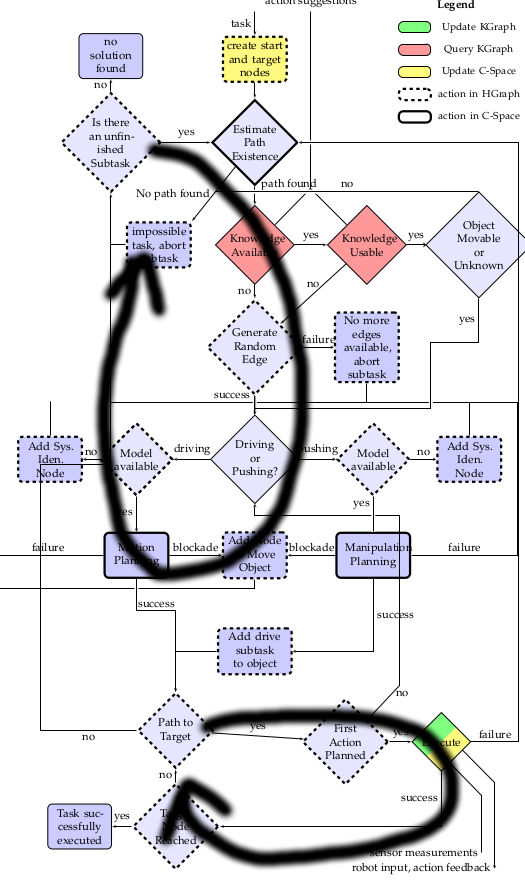
\includegraphics[width=7cm]{figures/two_loops_identified}
    \caption{The search (above) and execution (below) loop.}%
    \label{fig:two_loops_identified}
\end{figure}

Whilst the \ac{halgorithm} resides in the search loop, hypotheses are formed. Forming a hypothesis generates nodes, edges, and progressing their status as described in \cref{tikz:status_identification_edge,tikz:status_action_edge}. In the execution loop \textit{an edge is being executed}, a phrase to describe that the controller residing in an edge is sending control input toward the robot. The \ac{halgorithm} operates synchronously, thus at any point in time, the \ac{halgorithm} resides in a single block within \cref{tikz:flowchart_hgraph}. The result is that the robots cannot operate whilst the \ac{halgorithm} resides in the search loop, and during execution, no hypothesis can be formed or updated. Assumption~\ref{assumption:closed_world} guarantees that the robot environment does not change causing existing hypotheses to be outdated.\bs

\subsection{Examples}%
\label{subsec:hgraph_example}

Before displaying example \ac{hgraph}'s a legend is now presented.\bs

\begin{figure}[H]
    \centering
    \begin{subfigure}{0.2\textwidth}
    \centering
    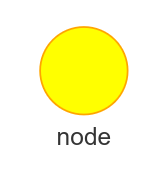
\includegraphics[width=0.7\textwidth]{figures/connecting_nodes/legend/node}
    \caption{Regular node created by the \ac{halgorithm}.\newline}%
    \end{subfigure}
    \begin{subfigure}{0.2\textwidth}
    \centering
    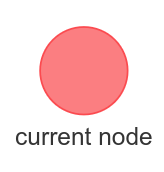
\includegraphics[width=0.7\textwidth]{figures/connecting_nodes/legend/current_node}
    \caption{Current node indicates that it's outgoing edge is now or is next to be executed.}%
    \end{subfigure}
    \begin{subfigure}{0.2\textwidth}
    \centering
    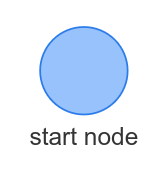
\includegraphics[width=0.7\textwidth]{figures/connecting_nodes/legend/starting_node}
    \caption{Starting node, one is generated at for every subtask.}%
    \end{subfigure}
    \begin{subfigure}{0.2\textwidth}
    \centering
    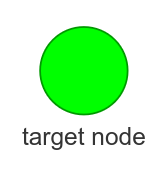
\includegraphics[width=0.7\textwidth]{figures/connecting_nodes/legend/target_node}
    \caption{Target node, one is generated for every subtask.\newline}%
    \end{subfigure}

    \begin{subfigure}{0.33\textwidth}
    \centering
    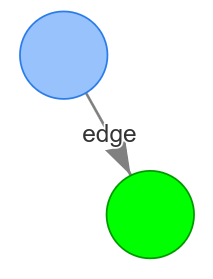
\includegraphics[width=0.7\textwidth]{figures/connecting_nodes/legend/edge}
    \caption{Edge with status IN, PE, SM, PP or EX.}%
    \end{subfigure}
    \begin{subfigure}{0.33\textwidth}
    \centering
    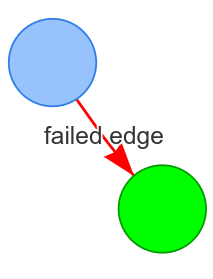
\includegraphics[width=0.7\textwidth]{figures/connecting_nodes/legend/failed_edge}
    \caption{Edge with status FAILED (FAIL)}%
    \end{subfigure}
    \begin{subfigure}{0.33\textwidth}
    \centering
    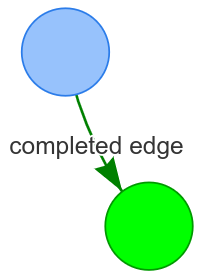
\includegraphics[width=0.7\textwidth]{figures/connecting_nodes/legend/completed_edge}
    \caption{Edge with status COMPLETED (CO)}%
    \end{subfigure}
    \caption{Legend for \ac{hgraph}'s nodes an edges}%
    \label{fig:hgraph_legend}
\end{figure}

\paragraph{Driving and Pushing} Four examples are presented, starting with a driving task in \cref{fig:robot_drive_hgraph}, then a pushing task in \cref{fig:robot_push_hgraph}.\bs

\begin{figure}[H]
    \centering
    \begin{subfigure}{.3\textwidth}
    \centering
    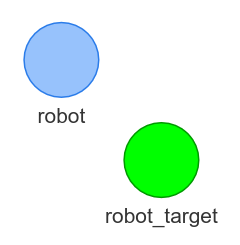
\includegraphics[width=0.7\textwidth]{figures/connecting_nodes/robot_to_target/robot_to_target}
    \end{subfigure}
    \begin{subfigure}{.3\textwidth}
    \centering
    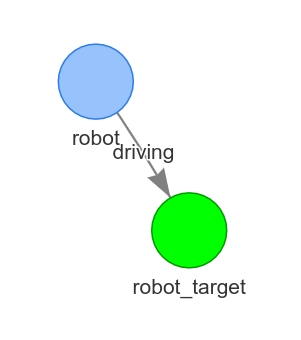
\includegraphics[width=0.9\textwidth]{figures/connecting_nodes/robot_to_target/robot_drive_target}
    \end{subfigure}
    \begin{subfigure}{.3\textwidth}
    \centering
    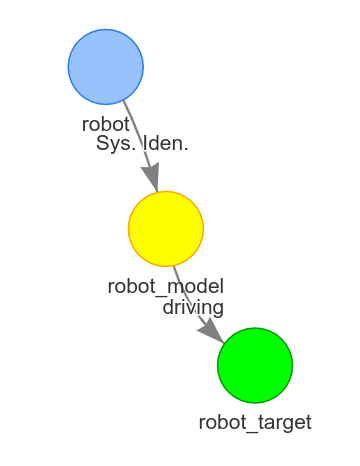
\includegraphics[width=\textwidth]{figures/connecting_nodes/robot_to_target/robot_iden_drive_target}
    \end{subfigure}
    \caption{\ac{hgraph} generated by the \ac{halgorithm} to drive the robot to a target configuration}%
    \label{fig:robot_drive_hgraph}
\end{figure}

The robot does not have a system model of itself, thus first system identification must be performed before it can drive to the specified target configuration. The \ac{kgraph} that will be discussed in \cref{subsec:kgraph_definition} can suggest an action that includes a system model. In that case, system identification is not needed. The following figure displays succesfully executing the hypothesis found in \cref{fig:robot_drive_hgraph}.\bs

\begin{figure}[H]
    \centering
    \begin{subfigure}{.3\textwidth}
    \centering
    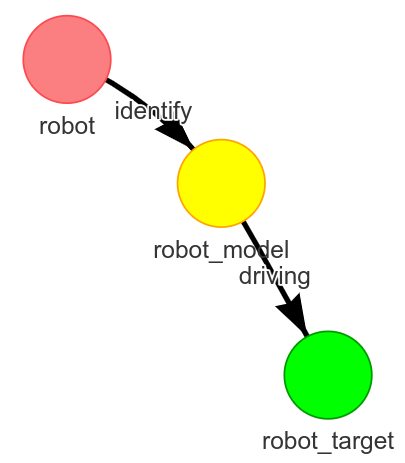
\includegraphics[width=0.8\textwidth]{figures/connecting_nodes/robot_to_target/execute_robot_to_target_1}
    \end{subfigure}
    \begin{subfigure}{.3\textwidth}
    \centering
    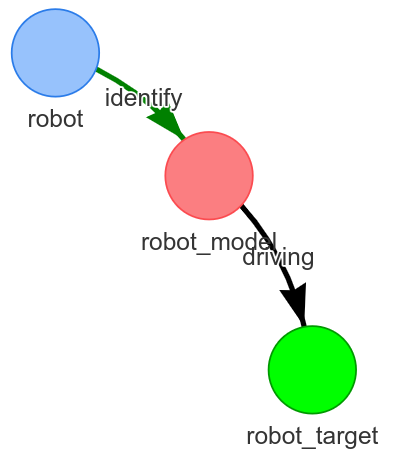
\includegraphics[width=0.8\textwidth]{figures/connecting_nodes/robot_to_target/execute_robot_to_target_2}
    \end{subfigure}
    \begin{subfigure}{.3\textwidth}
    \centering
    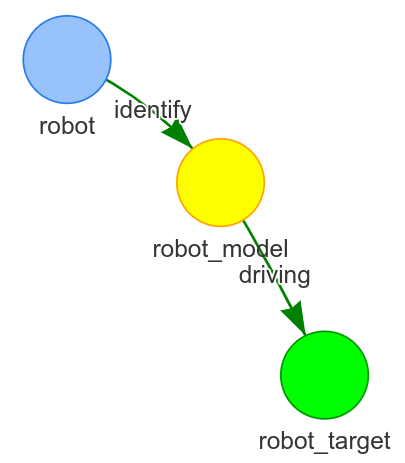
\includegraphics[width=0.8\textwidth]{figures/connecting_nodes/robot_to_target/execute_robot_to_target_3}
    \end{subfigure}
    \caption{Executing the hypothesis found in \cref{fig:robot_drive_hgraph}.}
    \label{fig:execute_robot_to_target}
\end{figure}

Upcoming figure will display the hypothesis generated to push an object to a target position. Both generating a hypothesis and executing the hypothesis are intertwined, this is because certain information should first be collected from the environment before the full hypothesis can be generated. An example is the \textit{best\_push\_position} that can be found in \cref{subfig:robot_push_7,subfig:robot_push_8,subfig:robot_push_9}. The \textit{best\_push\_position} can be found after manipulation planning for the pushing edge is completed. For motion planning a system model is required, thus the corresponding system identification edge should be completed before manipulation planning can start, and than the \textit{best\_push\_position} can be determined.\bs

\begin{figure}[H]
    \centering
    \begin{subfigure}{.3\textwidth}
    \centering
    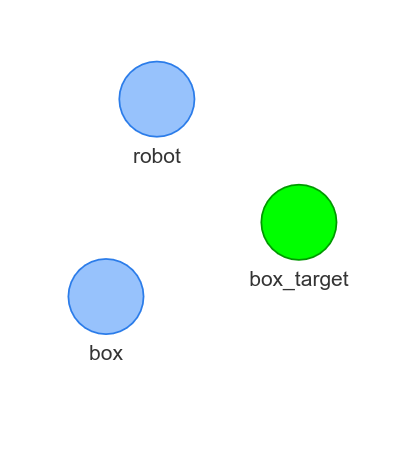
\includegraphics[width=0.8\textwidth]{figures/connecting_nodes/robot_push/robot_push_1}
    \caption{}
    \end{subfigure}
    \begin{subfigure}{.3\textwidth}
    \centering
    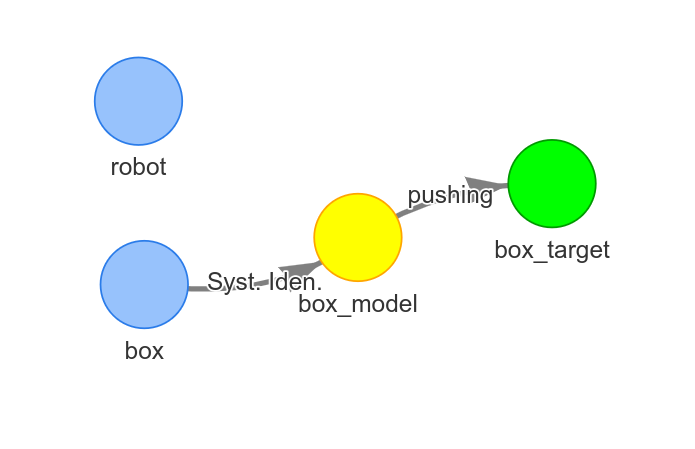
\includegraphics[width=1.1\textwidth]{figures/connecting_nodes/robot_push/robot_push_2}
    \caption{}\label{subfig:robot_push_2}
    \end{subfigure}
    \begin{subfigure}{.3\textwidth}
    \centering
    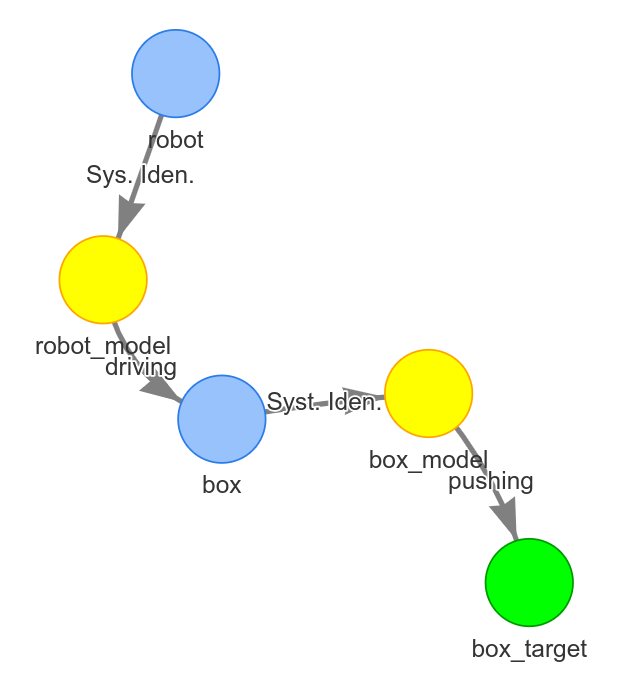
\includegraphics[width=1\textwidth]{figures/connecting_nodes/robot_push/robot_push_3}
    \caption{}\label{subfig:robot_push_3}
    \end{subfigure}

    \begin{subfigure}{.3\textwidth}
    \centering
    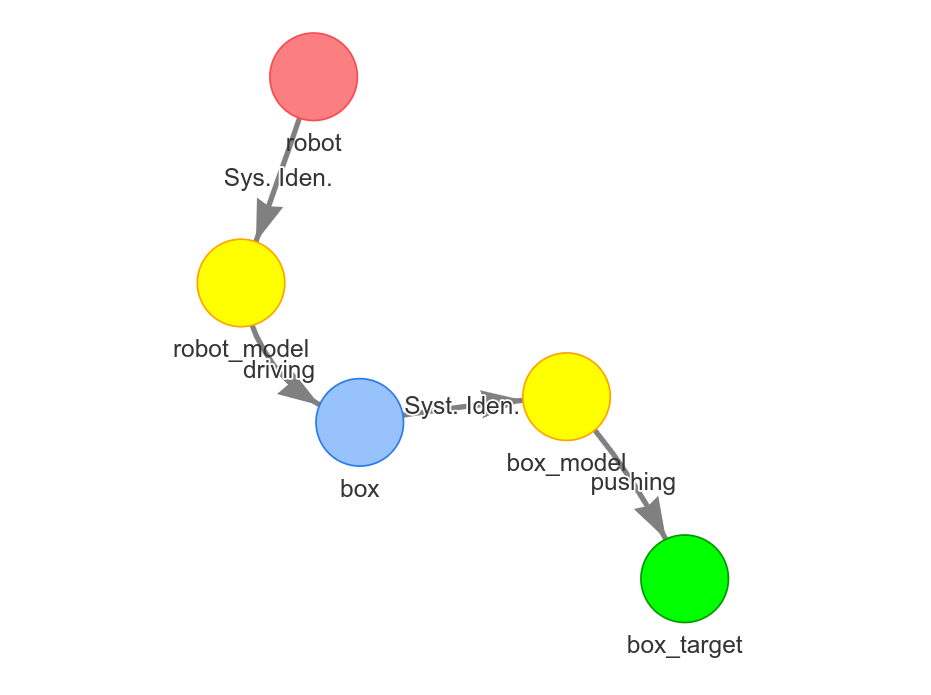
\includegraphics[width=1\textwidth]{figures/connecting_nodes/robot_push/robot_push_4}
    \caption{}\label{subfig:robot_push_4}
    \end{subfigure}
    \begin{subfigure}{.3\textwidth}
    \centering
    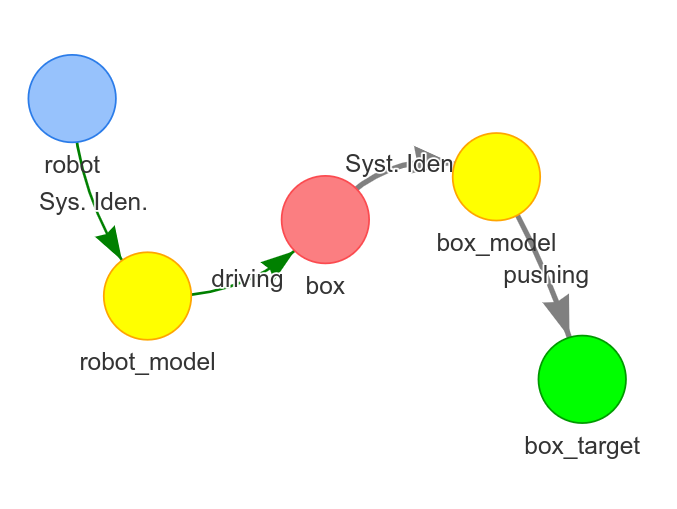
\includegraphics[width=1.05\textwidth]{figures/connecting_nodes/robot_push/robot_push_5}
    \caption{}\label{subfig:robot_push_5}
    \end{subfigure}
    \begin{subfigure}{.3\textwidth}
    \centering
    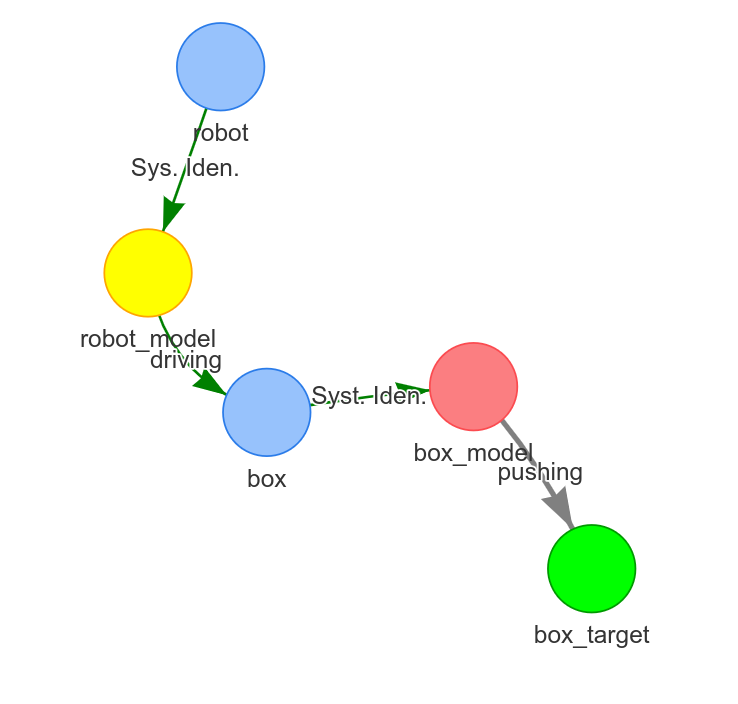
\includegraphics[width=1.05\textwidth]{figures/connecting_nodes/robot_push/robot_push_6}
    \caption{}\label{subfig:robot_push_6}
    \end{subfigure}

    \begin{subfigure}{.3\textwidth}
    \centering
    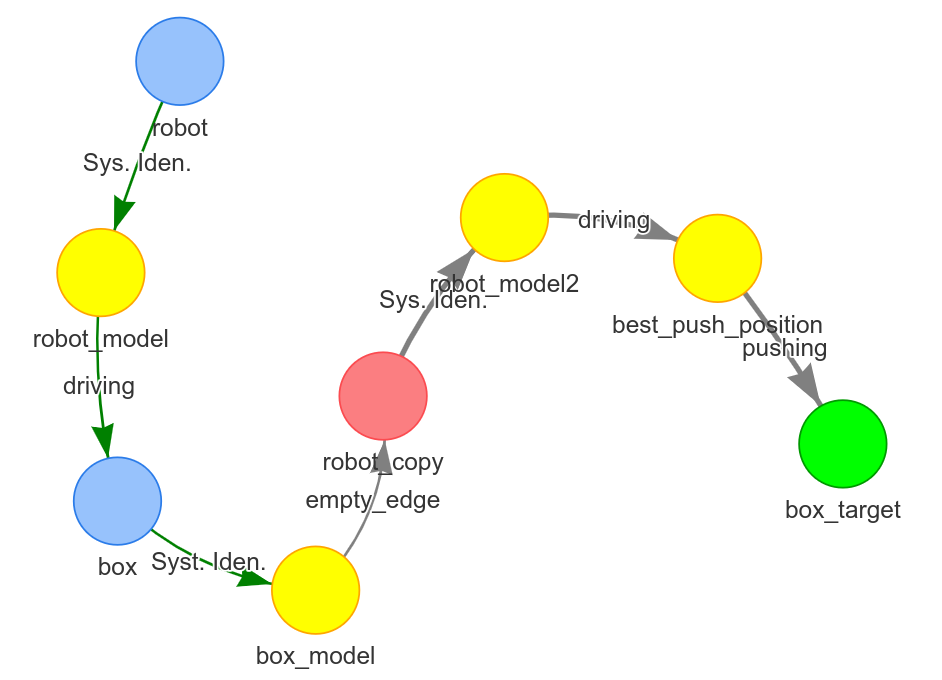
\includegraphics[width=1\textwidth]{figures/connecting_nodes/robot_push/robot_push_7}
    \caption{}\label{subfig:robot_push_7}
    \end{subfigure}
    \begin{subfigure}{.3\textwidth}
    \centering
    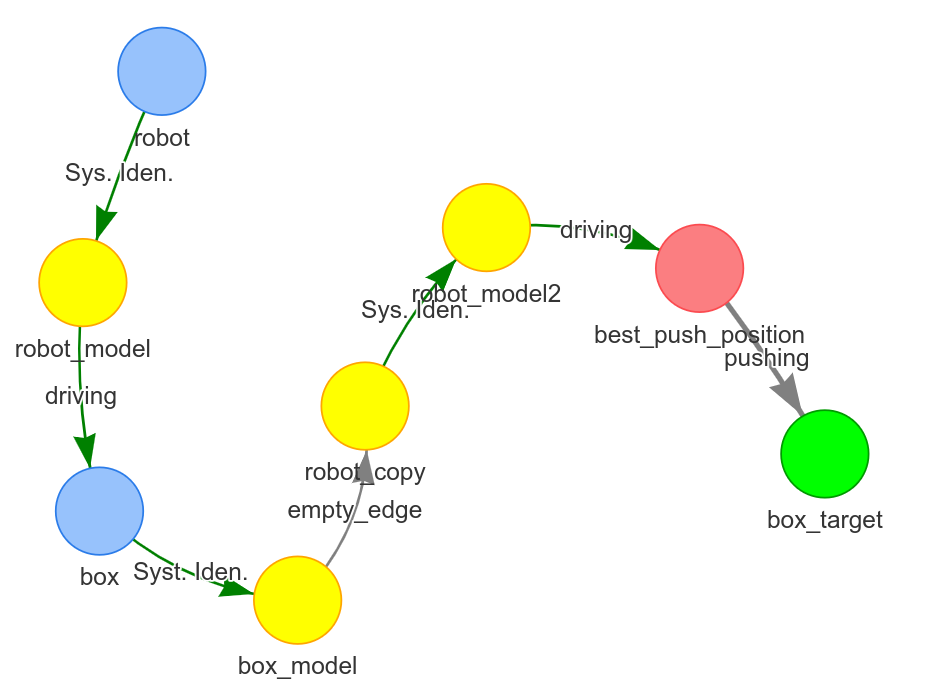
\includegraphics[width=1.05\textwidth]{figures/connecting_nodes/robot_push/robot_push_8}
    \caption{}\label{subfig:robot_push_8}
    \end{subfigure}
    \begin{subfigure}{.3\textwidth}
    \centering
    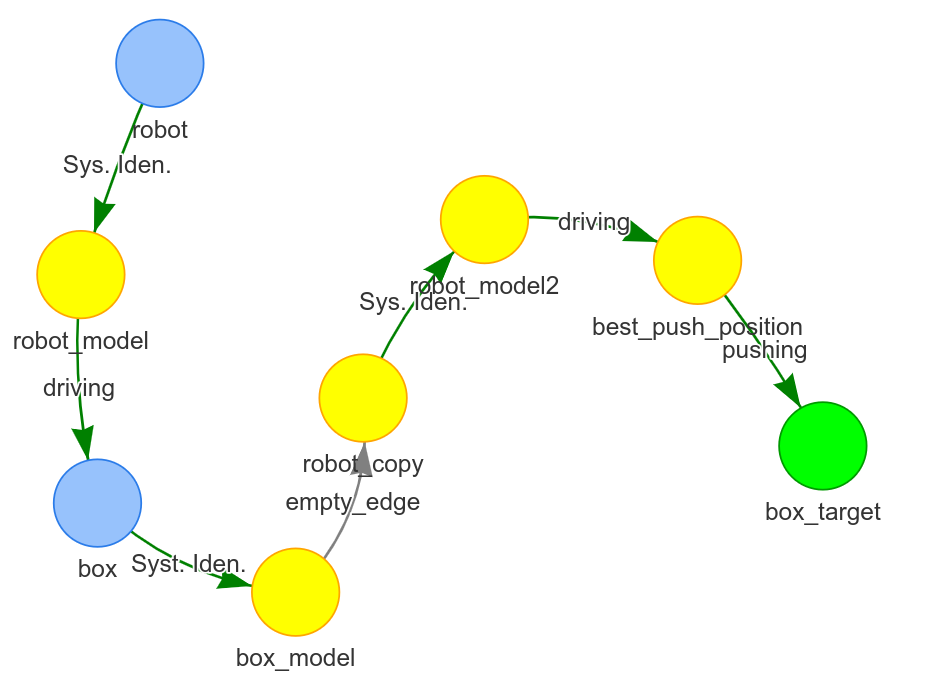
\includegraphics[width=1.05\textwidth]{figures/connecting_nodes/robot_push/robot_push_9}
    \caption{}\label{subfig:robot_push_9}
    \end{subfigure}
    \caption{\ac{hgraph} for pushing the green box to the target configuration}%
    \label{fig:robot_push_hgraph}
\end{figure}
Especially in \cref{subfig:robot_push_2,subfig:robot_push_3} the backward search is clearly visible, the \ac{halgorithm} searches from target node to the robot node. \Cref{fig:robot_push_hgraph} is extensive because every nessecary steps is included whilst some could be skipped. First, identifying a system model for robot driving twice, if the system model created in edge Sys. Iden. pointing toward node robot\_model is reused, then the edge Sys. Iden. pointing toward robot\_model\_1 would be unnecessary. Second, if system models would already be availeble for driving and pushing, no single system identification edge would be required. A \textit{empty\_edge} can be seen in \cref{subfig:robot_push_7,subfig:robot_push_8,subfig:robot_push_9}, the empty\_edge serves to connect a node to another node (box\_model to robot\_copy in \cref{fig:robot_push_hgraph}). The empty\_edge can be traversed without execution, holds no controller, system model or status.\bs

\paragraph{Encountering a Blocked Path}%
During propagation of an action edge's status, motion or manipulation planning occurs. If an object is blocking the path, planning will detect it and the \ac{halgorithm} tries to free the path. In the next example the \ac{halgorithm} detects a blocking object and frees the path by pushing the blocking object to a new configuration, and can be visulised in \cref{fig:blocking_obj_hgraph}.\bs

\begin{figure}[H]
    \centering
    \begin{subfigure}{.3\textwidth}
    \centering
    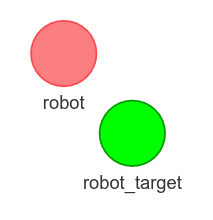
\includegraphics[width=0.5\textwidth]{figures/connecting_nodes/blocking_obj/blocking_obj_1}
    \caption{}
    \end{subfigure}
    \begin{subfigure}{.3\textwidth}
    \centering
    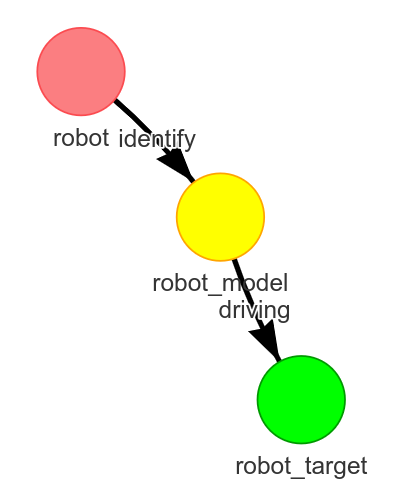
\includegraphics[width=\textwidth]{figures/connecting_nodes/blocking_obj/blocking_obj_2}
    \caption{}\label{subfig:blocking_obj_2}
    \end{subfigure}
    \begin{subfigure}{.3\textwidth}
    \centering
    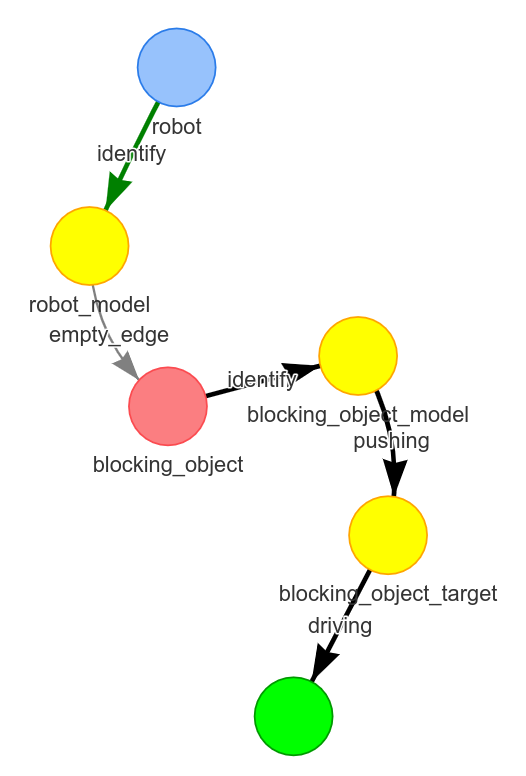
\includegraphics[width=\textwidth]{figures/connecting_nodes/blocking_obj/blocking_obj_3}
    \caption{}\label{subfig:blocking_obj_3}
    \end{subfigure}

    \begin{subfigure}{.3\textwidth}
    \centering
    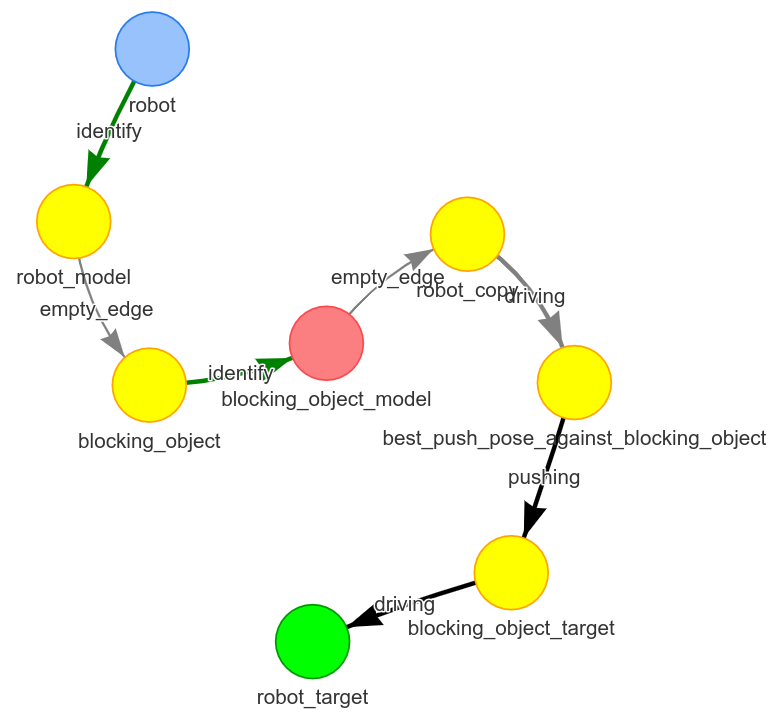
\includegraphics[width=1.3\textwidth]{figures/connecting_nodes/blocking_obj/blocking_obj_4}
    \caption{}\label{subfig:blocking_obj_4}
    \end{subfigure}
    \begin{subfigure}{.3\textwidth}
    \centering
    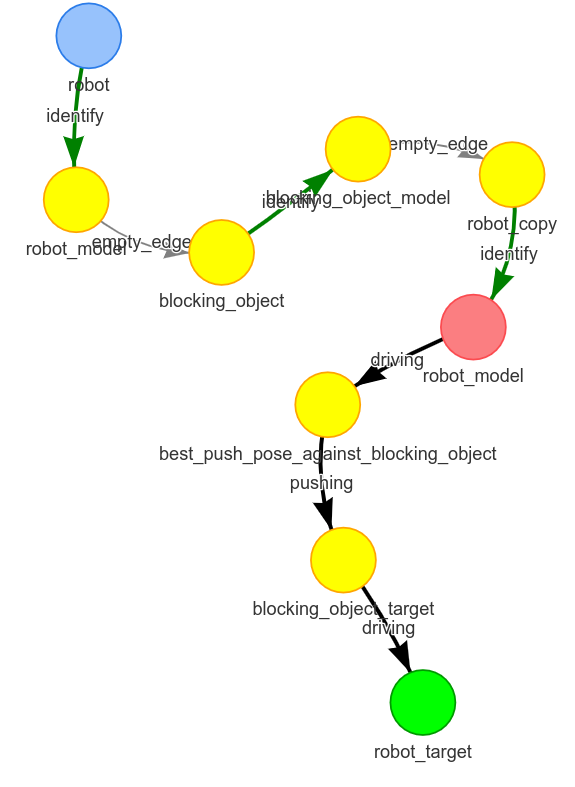
\includegraphics[width=\textwidth]{figures/connecting_nodes/blocking_obj/blocking_obj_5}
    \caption{}\label{subfig:blocking_obj_5}
    \end{subfigure}
    \begin{subfigure}{.3\textwidth}
    \centering
    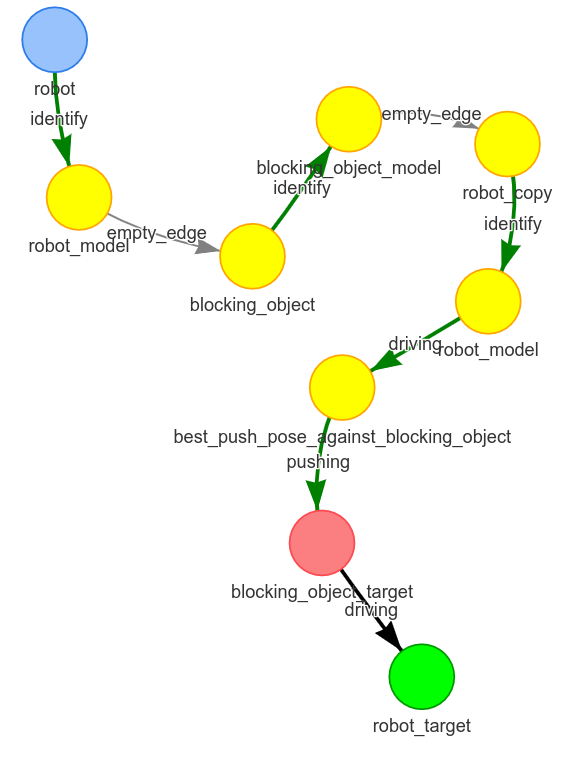
\includegraphics[width=\textwidth]{figures/connecting_nodes/blocking_obj/blocking_obj_6}
    \caption{}\label{subfig:blocking_obj_6}
    \end{subfigure}
    \caption{\ac{hgraph} for driving to target configuration and encountering a blocked path}%
    \label{fig:blocking_obj_hgraph}
\end{figure}

\paragraph{Encountering Failure}%
In the last example, the first hypothesis fails to complete and the \ac{halgorithm} tries to generate a new hypothesis that also fails to complete. Several faults and failures are modelled, the \ac{halgorithm} response to faults and failure is the same. If during the propagation of an edge's status any kind of failure arises, the failed edge and corresponding edges are marked as failed. Equally during execution, if a fault is detected, the execution halts and the edge and corresponding edges are marked as \quotes{failed}, the procedure can be seen in \cref{fig:failure_in_hgraph}.\bs

\begin{figure}[H]
    \centering
    \begin{subfigure}{.3\textwidth}
    \centering
    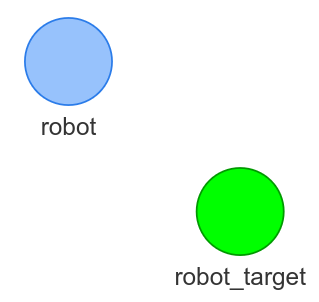
\includegraphics[width=0.8\textwidth]{figures/connecting_nodes/failure/fail_1}
    \end{subfigure}
    \begin{subfigure}{.3\textwidth}
    \centering
    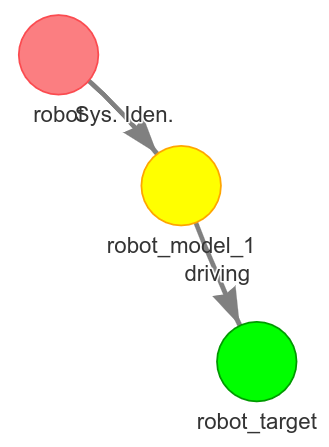
\includegraphics[width=1.1\textwidth]{figures/connecting_nodes/failure/fail_2}
    \end{subfigure}
    \begin{subfigure}{.3\textwidth}
    \centering
    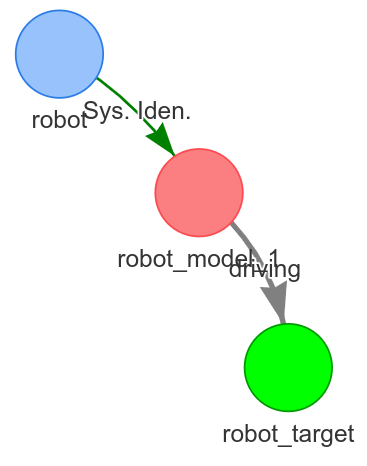
\includegraphics[width=1\textwidth]{figures/connecting_nodes/failure/fail_3}
    \end{subfigure}

    \begin{subfigure}{.3\textwidth}
    \centering
    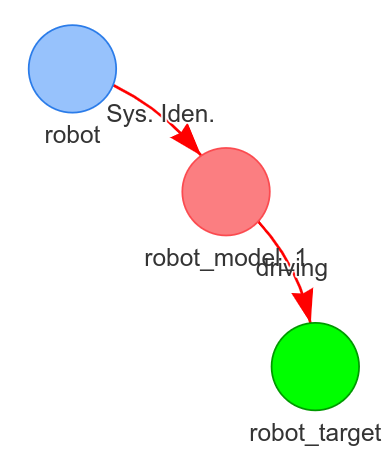
\includegraphics[width=1\textwidth]{figures/connecting_nodes/failure/fail_4}
    \end{subfigure}
    \begin{subfigure}{.3\textwidth}
    \centering
    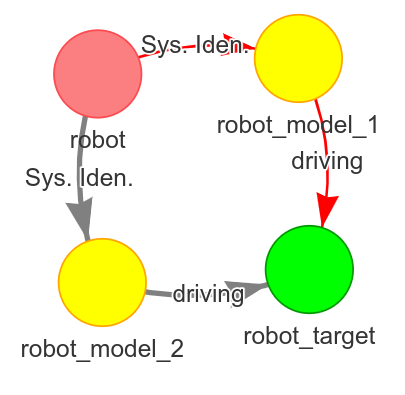
\includegraphics[width=1\textwidth]{figures/connecting_nodes/failure/fail_5}
    \end{subfigure}
    \begin{subfigure}{.3\textwidth}
    \centering
    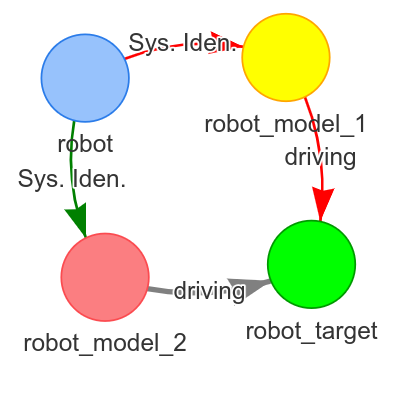
\includegraphics[width=1\textwidth]{figures/connecting_nodes/failure/fail_6}
    \end{subfigure}

    \begin{subfigure}{.3\textwidth}
    \centering
    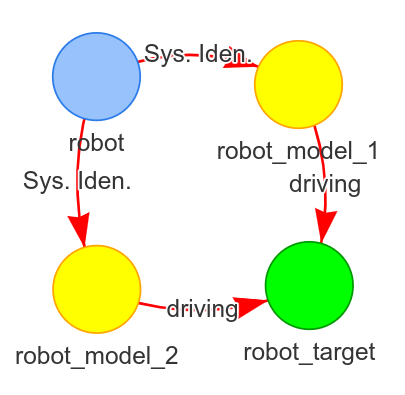
\includegraphics[width=1\textwidth]{figures/connecting_nodes/failure/fail_7}
    \end{subfigure}
    \hfill
    \caption{Executing two hypothesis, both failing to complete because a fault of failure emerged.}%
    \label{fig:failure_in_hgraph}
\end{figure}

In \cref{fig:failure_in_hgraph} only two parameterisations of drive controller and system model were available. Thus after two failed hypothesis the \ac{halgorithm} concludes it cannot complete this task.\bs


What by now hopefully became clear to the reader is that the \ac{hgraph} autonomously searches for hypotheses to solve the task, one subtask at a time. The \ac{hgraph} switches between the search and execution loop. Switching from the search loop toward the execution loop when a hypothesis is found, and switching back when a hypothesis is completed or an action failed to complete.\bs

The limited number of possible edges (every combination of a system identification method with a compatible control method) guarantees that the robot tries to connect 2 nodes, but concludes that it cannot reach a node if all possible edges have failed. Eventually running out of nodes to connect and conclude that a subtask cannot be completed.\bs

In the next section, the edges that are executed will be reviewed and stored in a knowledge base. The knowledge base will suggest edges when faced with similar nodes to connect.
\


\section{Knowledge Graph}%
\label{sec:kgraph}
The \ac{hgraph}, discussed in the previous section, spans a lifetime over a single task. In the \ac{hgraph} only the object class is stored for the lifetime of the \ac{hgraph}. When a task is completed, the \ac{hgraph} is deconstructed and learned objects classes are lost. The \ac{kgraph}'s responsibility is to store objects classes for future tasks, and to make an ordering in the edge parameterizations where a edge parameterization comprises of a controller and system model. Estimating which parameterization would be the best candidate is an entire field of research. In this thesis the ordering is made by collecting action feedback on executed action edges and summarizing that feedback in a single metric, the \textit{success factor}. This metric combines two metrics the \acl{PE} and the success-fail ratio of an edge parameterization.\bs

The name \quotes{\acl{kgraph}} originates from the environmental knowledge it contains and its graph structure. Both the \ac{hgraph} and \ac{kgraph} are newly proposed frameworks built from the ground up, with only inspiration from an already existing technique, a backward search. The \ac{kgraph} is in an early stage of development and does therefore not (yet) adhere to any standard that apply to knowledge bases, such as first order-logic~\cite{barwise_introduction_1977,rensink_representing_2004}, relational databases~\cite{atzeni_relational_1993} or more practical, a language such as prologe~\cite{wielemaker_swiprolog_2012}.\bs

\subsection{Definition}
\label{subsec:kgraph_definition}


\todo[inline]{this section}

\subsection{Edge Metrics}
\label{subsec:edge_metrics}
\subsection{Example}
\label{subsec:kgraph_example}



\newpage

\begin{figure}[H] \centering
  \begin{tikzpicture}[node distance = 4.5cm, line width=1pt]
    % Nodes
    \node [block, fill=green!50] (first) {Update existing edge with new feedback};
    
    % legend 
    \node[text width=2.8cm, yshift=1cm, right of=first, text centered, rounded corners, minimum height=1em, label={[name=lab, yshift=0.4cm, left]\textbf{Legend}}, node distance=7cm] (legend1) {\small Update KGraph};
    \node[rectangle, draw, left of=legend1, fill=green!50, rounded corners, minimum height=1em, minimum width=1cm, node distance=2cm] (legend1color) {};
    \node[text width=2.8cm, below of=legend1, text centered, minimum height=1em, node distance=0.7cm] (legend2) {\small Query KGraph};
    \node[rectangle, draw, left of=legend2, fill=red!40, rounded corners, minimum height=1em, minimum width=1cm, node distance=2cm] (legend2color) {};
   
    
    % nodes, first row 
    \node [decision, below of=first, node distance=4.5cm, fill=red!40, text width=7.0em] (has_controller) {Does this parameterization exist in one of the center node's outgiong edges?};
    \node [block, left of=has_controller, fill=green!50] (new_transition) {Generate new edge with feedback edge with feedback existing node};
    
    % nodes, second row 
    \node [decision, fill=red!40, below of=has_controller, node distance=6cm, text width=6.0em] (obj_exist) {Does this object exist in a center node in the \ac{kgraph}?};

  \node [decision, fill=red!40, right of=obj_exist, node distance=4.5cm, text width=6.0em] (obj_exist2) {Does this object exist in a center node in the \ac{kgraph}?};
    \node [block, yshift=-3cm, above= of obj_exist2, node distance=-1.8cm] (send_feedback) {Send ordered list with controllers and models};
    
    \node [block, fill=green!50, left of=obj_exist] (new_object) {Generate new center node, side node and an edge with feedback};
    \node [block, right of=obj_exist2, node distance=3.8cm] (no_obj) {send empty list};
   
    % Edges
    \draw[stealth-] (obj_exist) -- node[left, at end]{action feedback} +(0,-3.5cm);
    \draw[-stealth] (obj_exist.west) -- node[above]{no} (new_object.east);
    \draw[-stealth] (obj_exist.north) -- node[left]{yes} (has_controller.south);
    \draw[-stealth] (has_controller.north) -- node[left]{yes} (first.south);
    \draw[-stealth] (has_controller.west) -- node[above]{no} (new_transition.east);
    
    \draw[-stealth] (obj_exist2.east) -- node[above]{no} (no_obj.west);
    \draw[-] (no_obj.east) -- +(0.7cm, 0);
    \draw[stealth-] (obj_exist2) -- node[left, at end]{action suggestion?} +(0,-3.5cm);
    \draw[-stealth] (obj_exist2.north) -- node[left]{yes} (send_feedback.south);
    \draw[-stealth] (send_feedback.east) -| node[at end, left]{action suggestion} +(4.5cm, -8.4cm);
\end{tikzpicture}
\caption{Flowchart displaying the knowledge graph's workflow.}%
\label{figure: flowchart_kgraph} 
\end{figure}



% \subsection{Edge Metrics}%
% \label{subsec:edge_metrics}
% \todo{Corrado: rephrase good and bad to sound like a professional cunt}
% The \ac{kgraph} keeps an ordered list of `good' and `bad' edge arguments (controller and system model). `Good' and `bad' are defined by edge metrics; these metrics are created after the completion of an edge, regardless of whether the edge was completed or failed. An indication is given on why specific metrics matter in \Cref{table:review_edge_metrics}.

% \noindent
% \begin{table}[H]
% \centering
% \begin{tabular}%
% {>{\raggedright\arraybackslash}p{0.25\textwidth}%
% >{\raggedright\arraybackslash}p{0.65\textwidth}}
% \acf{PE}&  To better compare prediction errors the \ac{PE} is summarized and average \ac{PE}. The average \ac{PE} indicates an accurate system model but can give misleading results since \ac{PE} is also an indicator of unexpected collisions. Prediction error should thus only be used if there are no collisions detected. The average \ac{PE} has more flaws since outliers mostly determine the average. For the largest part, some unfortunate outliers in the \ac{PE} might determine the average \ac{PE}. The average \ac{PE} will thus not be used because it is not robust enough.\\
% % \acf{TE}& For a low \ac{TE}, the system model must be close to the real motion equations to yield a feasible path, the controller must be well tuned to be able to track that path and the controller and system model must be in collaboration, because the controller uses the system model to calculate system input. A low \ac{TE} tells multiple things, whilst a high \ac{TE} would indicate improvements could be gained in the controller, the system model or their collaboration.\\
% ratio num\_succesfully completed edges and num\_total edges & Over time, the \ac{kgraph} can recommend the same edge arguments multiple times. Logging the ratio of succeeding edges vs total edges builds an evident portfolio. Still, this metric has to be taken with a grain of salt because edges with equal edge arguments perform similar actions e.g.~pushing an object through a wide corridor is compared to pushing the same object through a narrow corridor. One could say \quotes{comparing apples with pears}\todo{Corrado: But then you would have task-specific metrics right? Meaning a knowledge graph for when you do pushes in open space and one for small corridors? I don’t know if this would scale. To make sense of the metric this metric should be task specific though }.\\
% the final position and \newline displacement error & The quality of the result is measured in the final position and displacement error. The importance should thus be stressed when ordering edge arguments.\\
% planning time& With system identification, path estimation, motion or manipulation planning, the planning time can vary in orders of magnitude between simple or more complex approaches.\\
% run time& Also known as execution time, would be a quality indicator if start- and target states were equal. Edges are recommended to solve similar tasks where the path length between the start and target state differs. Thus planning time is not of any use to rank edges.\\
% completion time = \newline run time + planning time & With the same argumentation as run time, completion time is not used to rank edges.\\
% \end{tabular}
% \caption{The edge metrics employed to establish a ranking of edge parameterizations.}
% \label{table:review_edge_metrics}
% \end{table}

% \todo{Corrado: So why do we have all these metrics if you do not consider them? Shouldn’t you normalize the metrics such that they are at least comparable with each other in similar yet differe tasks?}



\section{Benchmark Tests}
\label{section: btests}
This section gives insight how the proposed method improves upon methods proposed by existing literature. An improvement is presented with an elaborate example, called a benchmark tests. The benchmark tests, BTests for short include an image of the starting environment, a description of the task, the final knowledge graph and a hypothesis graph which should be generated once the algorithm is implemented. The hypothesis graph may skip certain steps which are not the focus the BTest, and would only clutter the HGraph. \\

Once again the legend for a HGraph is displayed.\\

\begin{figure}[H]
     \centering
     \begin{subfigure}[b]{0.5\textwidth}
         \centering
         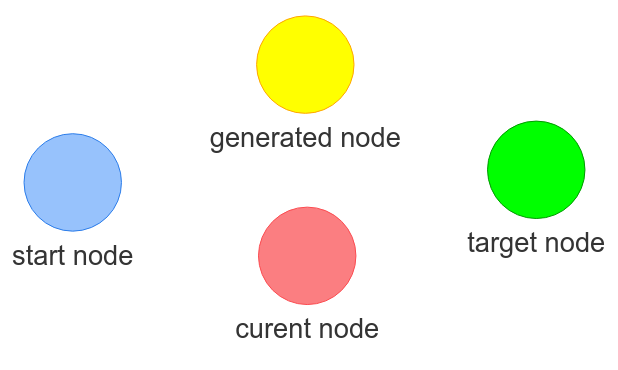
\includegraphics[width=\textwidth]{figures/hgraph_legend_nodes.png}
         \caption{4 nodes used in the HGraph, \textbf{\large Node labels with R:, M: or RM: indicate that the robot is present in the node (R), a model is available (M)}}
     \end{subfigure}
     
     \begin{subfigure}[b]{0.49\textwidth}
         \centering
         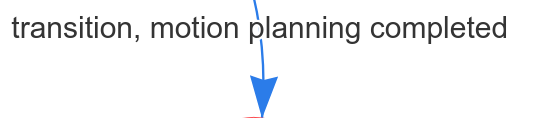
\includegraphics[width=\textwidth]{figures/hgraph_legend_transition1.png}
         \caption{Arrow with solid line}
     \end{subfigure}
    \hfill 
    \begin{subfigure}[b]{0.49\textwidth}
         \centering
         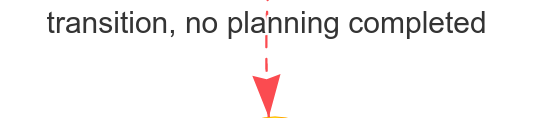
\includegraphics[width=\textwidth]{figures/hgraph_legend_transition2.png}
         \caption{Arrow with dashed line}
     \end{subfigure}
   \caption{HGraph Legend}
    \label{figure: hgraph_legend2}
\end{figure}


\subsection{Blockade by the Duck}
\Cref{figure: blockade_by_duck} displays a robot, 3 unmovable walls, a movable yellow duck and a movable red cube. \textbf{The task} given to the robot is to place the red cube inside the walls. The duck is "guarding" the target location of the red cube. The robot has to first detect, and then to take care of the duck by pushing it to a unspecified location such that the cube can pass through. It is assumed that there is enough space around the objects for system identification, alternatively system identification could be performed on the individual objects, and then perform the blockade by duck task. This BTest already involves many different aspects. Such as system identification on the robot itself, the red cube, the green wall and the duckling, motion planning, manipulation planning and replanning. The goal of this BTest is to give insight that the proposed methods can do all these different aspects.

\begin{figure}[H]
    \centering
    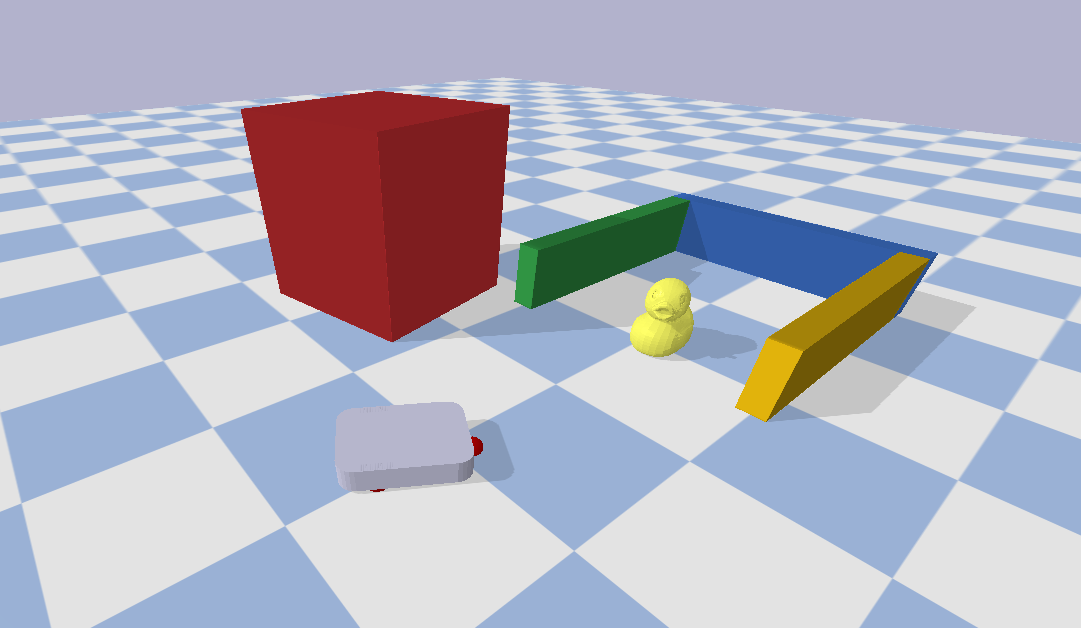
\includegraphics[width=0.6\textwidth]{figures/blockade/blockade_by_duck.png}
    \caption{The robot is tasked with placing the cube inside the walls, only this is guarded by a duckling.}
    \label{figure: blockade_by_duck}
\end{figure}

\begin{figure}[H]
     \centering
     \begin{subfigure}[b]{0.49\textwidth}
         \centering
         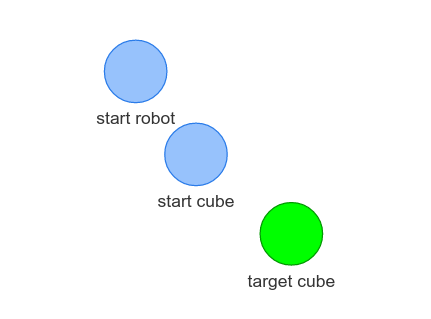
\includegraphics[width=\textwidth]{figures/blockade/1.png}
         \caption{Creating starting and target nodes}
     \end{subfigure}
     \hfill
     \begin{subfigure}[b]{0.49\textwidth}
         \centering
         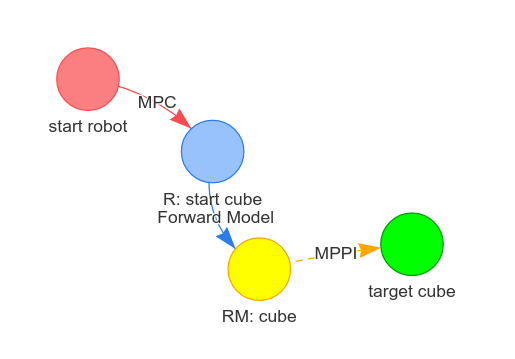
\includegraphics[width=\textwidth]{figures/blockade/2.png}
         \caption{Generate transitions and set start robot as current node}
     \end{subfigure}
     
     \begin{subfigure}[b]{0.49\textwidth}
         \centering
         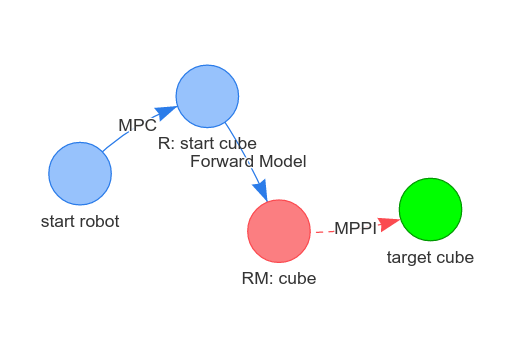
\includegraphics[width=\textwidth]{figures/blockade/3.png}
         \caption{Execute first 2 transitions}
     \end{subfigure}
     \hfill
     \begin{subfigure}[b]{0.49\textwidth}
         \centering
         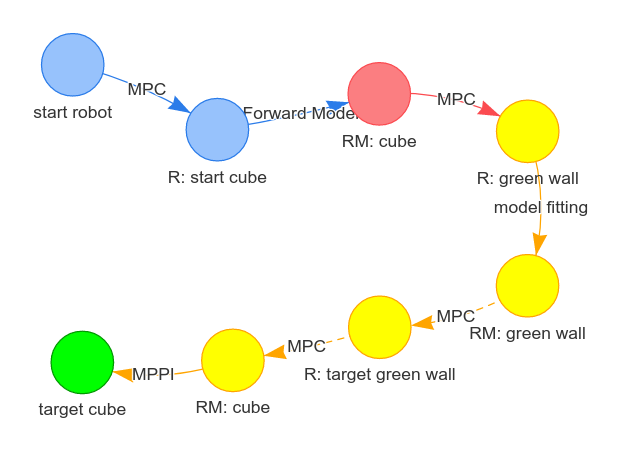
\includegraphics[width=\textwidth]{figures/blockade/4.png}
         \caption{In manipulation a subtask is created to move the green wall, these transitions are expected to complete successfully, completing the task}
     \end{subfigure}
     \caption{HGraph generating hypothesis to push the unmovable green wall and then push the cube to the target position. The figure continues on the next page. For the legend, see \cref{figure: hgraph_legend}}
     \label{figure: blockade_hgraph_first}
\end{figure}

As can be seen in \cref{figure: blockade_hgraph_first}, the HGraph has planned to push the cube toward the target position over the shortest path. On this path the (up to now) unknown green wall stands which needs to be moved before the cube can be pushed toward it's target position. The green wall needs to be pushed such that is does not intersect with the planned path for the cube. \\

The HGraph displayed in \cref{figure: blockade_hgraph_first,figure: blockade_hgraph_second} skips multiple steps in order to focus on the important steps. One of these skipped steps for example is system identification to find a model for the robot itself or the removal of insignificant nodes. 

\begin{figure}[H]
     \centering
     \begin{subfigure}[b]{0.49\textwidth}
         \centering
         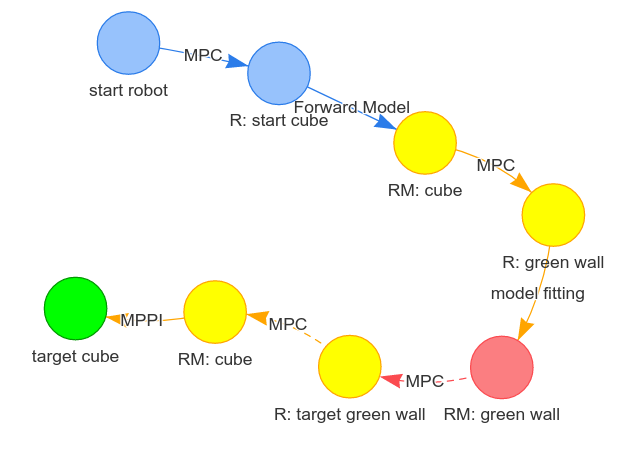
\includegraphics[width=1\textwidth]{figures/blockade/5.png}
         \caption{Robot drives to green wall and performs system identification}
     \end{subfigure}
     \hfill
     \begin{subfigure}[b]{0.49\textwidth}
         \centering
         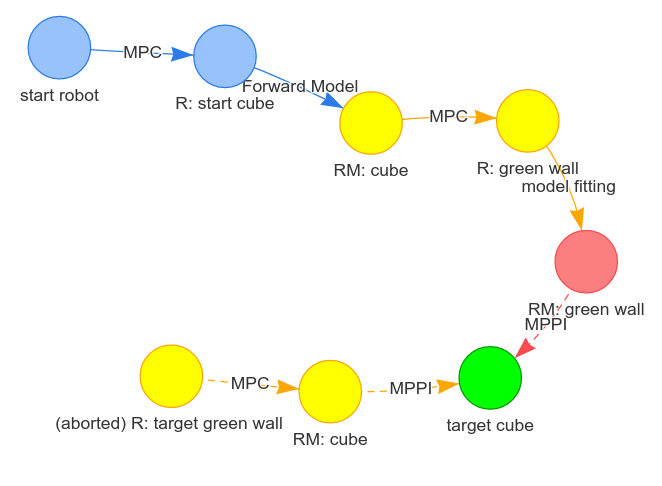
\includegraphics[width=\textwidth]{figures/blockade/6.png}
         \caption{Green wall appears to be unmovable, pushing the green wall is impossible, abort subtask to push green wall to target position}
     \end{subfigure}

     \begin{subfigure}[b]{0.49\textwidth}
         \centering
         \includegraphics[width=\textwidth]{figures/blockade/7.png}
         \caption{Generate a new starting state since much in the environment has now changed, replan a path from starting to target node}
     \end{subfigure}
     \hfill
     \begin{subfigure}[b]{0.49\textwidth}
         \centering
         \includegraphics[width=\textwidth]{figures/blockade/8.png}
         \caption{Execute new plan to push the duck and then push the cube to the target position}
     \end{subfigure}
     \caption{HGraph detecting that the green wall is unmovable, generate new hypothesis pushing the movable duck and then push the cube to the target position, For the legend, see \cref{figure: hgraph_legend2}}
     \label{figure: blockade_hgraph_second}
\end{figure}

The proposed approach and expected HGraph tackles a problem which \cite{siciliano_path_2009,wang_affordance-based_2020,scholz_navigation_2016} are not able to solve because they lack a crucial component. \cite{siciliano_path_2009} can navigate through movable obstacles and place objects on target positions. It is however provided with a set of movable and unmovable obstacles, the lack of learning dynamics prevents adaptation to new or changed environments. \cite{wang_affordance-based_2020} is able to navigate among movable obstacles and where required, identify if an object is pushable and if so, push an object to free it's path. A push to free the path is quite different from pushing to a target position. Lacking is thus the ability to manipulate objects to target positions, which is required in the blockade by duck task. The same argument holds for \cite{scholz_navigation_2016} who can navigate and move an object to free the path, but is unable to manipulate an object toward a target position. \\

\begin{figure}[H]
    \centering
    \includegraphics[width=0.6\textwidth]{figures/blockade/blockade_kgraph.png}
    \caption{Knowledge graph after completion of the blockade task.}
    \label{figure: blockade_kgraph}
\end{figure}

\subsection{Surrounded by Cubes}
\Cref{figure: surrounded_by_boxes} displays a robot and 6 cubes, only the green cube is movable, the red, blue and yellow cubes are unmovable. \textbf{The task} given to the robot is to go toward a target location outside of the surrounding boxes. It is assumed that to drive toward target location the robot has to move a cube, moving the red cube gives the shortest path toward the target position, moving the blue cube gives a longer shortest path and moving the green cube gives an even longer shortest path. The goal of this BTest is to show that learned knowledge is stored and makes a difference when encountering objects for the second time. 

\begin{figure}[H]
    \centering
    \includegraphics[width=0.6\textwidth]{figures/surrounded/surrounded_by_boxes.png}
    \caption{The robot is tasked with going to a target position outside the surrounding boxes, only one box is movable}
    \label{figure: surrounded_by_boxes}
\end{figure}

\begin{figure}[H]
     \centering
     \begin{subfigure}[b]{0.49\textwidth}
         \centering
         \includegraphics[width=\textwidth]{figures/surrounded/1.png}
         \caption{Creating starting and target node}
     \end{subfigure}
     \hfill
     \begin{subfigure}[b]{0.49\textwidth}
         \centering
         \includegraphics[width=\textwidth]{figures/surrounded/2.png}
         \caption{Generate hypothesis driving toward target position and perform system identification on robot}
     \end{subfigure}
     
     \begin{subfigure}[b]{0.49\textwidth}
         \centering
         \includegraphics[width=\textwidth]{figures/surrounded/3.png}
         \caption{Find red cube blocking the path which needs to be moved}
     \end{subfigure}
     \hfill
     \begin{subfigure}[b]{0.49\textwidth}
         \centering
         \includegraphics[width=\textwidth]{figures/surrounded/4.png}
         \caption{Drive toward red cube and perform system identification}
     \end{subfigure}
     \begin{subfigure}[b]{0.49\textwidth}
         \centering
         \includegraphics[width=1\textwidth]{figures/surrounded/5.png}
         \caption{The red cube in unmovable, abort subtask and replan to move the blue cube}
     \end{subfigure}
     \hfill
     \begin{subfigure}[b]{0.49\textwidth}
         \centering
         \includegraphics[width=\textwidth]{figures/surrounded/6.png}
         \caption{Drive toward blue cube and perform system identification}
     \end{subfigure}
     \caption{Figure continues on the next page}
\end{figure}

\begin{figure}[H]
    \ContinuedFloat
     \begin{subfigure}[b]{0.49\textwidth}
         \centering
         \includegraphics[width=\textwidth]{figures/surrounded/7.png}
         \caption{Blue cube is unmovable, abort subtask and replan to move the green cube}
     \end{subfigure}
     \hfill
     \begin{subfigure}[b]{0.49\textwidth}
         \centering
         \includegraphics[width=\textwidth]{figures/surrounded/8.png}
         \caption{Green cube is movable, after system identification push it. Now the path is free to drive toward the robot's target position}
     \end{subfigure}
     \caption{After multiple failed hypothesis, a succeeding hypothesis is found which completes the task. For the legend, see \cref{figure: hgraph_legend2}.}
     \label{figure: surrounded_hgraph_second}
\end{figure}

\begin{figure}[H]
    \centering
    \includegraphics[width=0.7\textwidth]{figures/surrounded/surrounded_kgraph.png}
    \caption{Knowledge graph after completion of the surrounded task.}
    \label{figure:  surrounded_kgraph}
\end{figure}

\begin{figure}[H]
    \centering
    \includegraphics[width=0.5\textwidth]{figures/surrounded/thank_you_hgraph.png}
    \caption{The hypothesis graph after redoing the same surrounded task for the second time. For the legend, see \cref{figure: hgraph_legend2}.}
    \label{figure: surrounded_with_prior_knowledge}
\end{figure}

The second time the same surrounded task given to the robot some crucial knowledge is captured by the knowledge graph. Prior knowledge about the movability of the red, blue and green cubes is provided and system models for the cubes an the robot. as can be seen in \cref{figure: surrounded_with_prior_knowledge} immediately goes for pushing the movable cube to then drive toward the target position.

\subsection{Swapping Objects}
\Cref{figure: swap_hgraph} displays a robot and movable obstacles. \textbf{The task} given to the robot is to swap the two objects, the duck must go to the position where the cube currently is and vise versa. The goal of this BTest is to give insight into the proposed methods ability to handle multiple objects, and to show that hierarchical methods yields a suboptimal solution. \\

\begin{figure}[H]
    \centering
    \includegraphics[width=0.6\textwidth]{figures/swap/swap_obstacles.png}
    \caption{The robot is tasked with swapping the two obstacles}
    \label{figure: swap_obstacles}
\end{figure}

\begin{figure}[H]
     \centering
     \begin{subfigure}[b]{0.49\textwidth}
         \centering
         \includegraphics[width=\textwidth]{figures/swap/1.png}
         \caption{Creating starting and target nodes}
     \end{subfigure}
     \hfill
     \begin{subfigure}[b]{0.49\textwidth}
         \centering
         \includegraphics[width=\textwidth]{figures/swap/2.png}
         \caption{Generate hypothesis to perform system identification on duck and place duck on target position}
     \end{subfigure}
     \caption{Figure continues on the next page}
\end{figure}

\begin{figure}[H]
    \ContinuedFloat
     \begin{subfigure}[b]{0.49\textwidth}
         \centering
         \includegraphics[width=\textwidth]{figures/swap/3.png}
         \caption{Execute first 3 transitions}
     \end{subfigure}
     \hfill
     \begin{subfigure}[b]{0.49\textwidth}
         \centering
         \includegraphics[width=\textwidth]{figures/swap/4.png}
         \caption{The cube is a obstacle which needs to be moved during planning the duck to target position}
   \end{subfigure}
   
    \begin{subfigure}[b]{0.49\textwidth}
         \centering
         \includegraphics[width=\textwidth]{figures/swap/5.png}
         \caption{Execute transitions up until placing the duck on the target position}
     \end{subfigure}
     \hfill
     \begin{subfigure}[b]{0.49\textwidth}
         \centering
         \includegraphics[width=\textwidth]{figures/swap/6.png}
         \caption{Create hypothesis to place cube on target position and drive toward cube}
     \end{subfigure}
     \caption{Swapping two objects, for the legend, see \cref{figure: hgraph_legend2}.}
     \label{figure: swap_hgraph}
\end{figure}

\begin{figure}[H]
    \centering
    \includegraphics[width=0.6\textwidth]{figures/swap/swap_kgraph.png}
    \caption{Knowledge graph after completion of the swap task.}
    \label{figure: swap_kgraph}
\end{figure}

The expected HGraph shows promising results, the ability to handle multiple objects of which the start and target positions are overlapping. Whilst object rearrangement algorithms exists \cite{krontiris_dealing_2015}, only \cite{sabbagh_novin_model_2021} implements target positions of environment objects, it however only considers a single object and a free path. Allowing to conclude that learning object dynamics \textit{and} \ac{NAMO} \textit{and} specifying objects target positions is a fairly new area of robotics. \\

A limitation due to the hierarchical search in the HGraph becomes visible. Imagine the objects to be swapped are very far apart. The proposed solution drives (possibly whilst being closer to the cube) to the starting position of the duck then to the cube, moves the cube a bit, back to the duck, then push the duck to target position and finally push cube to target position. Worst case, the robot is driving the distance between both starting positions 5 times, optimal is less than 3 times (assuming the robot is less than the initial cube-duck distance from either the duck or the cube). \cite{goldberg_asymptotically_2020} already emphasised the suboptimality of hierarchical solutions. In addition, model mismatch and failure to find the existing path during motion and manipulation planning decrease the optimality of the plan found by the proposed method. Suboptimality is acceptable since that is not the goal of the literature study.







\section{Discussion}
\label{section: proposed_method_discussion}
The general structure of the hypothesis- and knowledge graph have been displayed in \cref{figure: flowchart_hgraph,figure: flowchart_kgraph}, the required components are listed, and benchmark tests display the expected outcome for specific situations and tasks. With a given task the robot will search for an action sequence to complete the task, upon failure of planning, generating new transitions or failure of execution, the robot will retry to find a different path toward completion of the given task. Executed transitions receive feedback which is processed in the knowledge graph. After trying all possibilities without success, the robot concludes it cannot find a solution to the task. \\

\Cref{table: compare_results} compares the expected results with recent literature. As can be seen, only \cite{sabbagh_novin_model_2021} is able to place objects on target positions \textit{and} learn object dynamics, however \cite{sabbagh_novin_model_2021} searches directly in a joint configuration space which is very different approach compared to the proposed solution. The proposed solution theoretically can navigate among movable objects \textit{and} put an object on target location \textit{and} learn object dynamics, which is the main contribution, to combine both 3 with a hierarchical solution.

\begin{table}[H]
    \centering
     \rowcolors{2}{white}{myEvenLighterColor}
    \begin{tabular}{c|c|c|c|c}
      Citation & \ac{NAMO} & \shortstack[]{Specify object\\target positions} & \text{manipulation} & \shortstack[]{Learns object\\dynamics}\\ \hline
    \cite{sabbagh_novin_model_2021} & \cmark & \cmark & \shortstack[]{driving, grasp-push,\\grasp-pull} & \cmark\\
    \cite{wang_affordance-based_2020} & \cmark & \xmark & \shortstack[]{driving, pushing} & 
    \cmark\\
    \cite{scholz_navigation_2016} & \cmark & \xmark & \shortstack[]{driving, pushing} & \cmark\\
    \cite{siciliano_path_2009} & \cmark & \xmark & \shortstack[]{driving,gripping} & \xmark\\
    \cite{goldberg_asymptotically_2020} & \cmark & \cmark & \shortstack[]{driving,gripping} & \xmark\\
    
    proposed solution & \cmark & \cmark & \shortstack[]{driving, pushing} & \cmark\\
    \end{tabular}
    \caption{Comparing the proposed method to recent literature}
    \label{table: compare_results}
\end{table}


